\documentclass[12pt,a4paper,twoside]{book}

%%%%%%%%%%%%%%%%%%%%%%%%%%%%%%%%%%%%%%%%%%%%%%%%%%%%%%%%%%%%%%%%%%%%%%%%
%%%%%%%%%%%% Packages %%%%%%%%%%%%%%%%%%%%%%%%%%%%%%%%%%%%%%%%%%%%%%%%%%
%%%%%%%%%%%%%%%%%%%%%%%%%%%%%%%%%%%%%%%%%%%%%%%%%%%%%%%%%%%%%%%%%%%%%%%%

% Do not modify the next 10 lines
% ------------------------------
%%%%%%
% In general useful packages
%%%%%%
\usepackage{ucs} 
\usepackage[utf8]{inputenc}  
\usepackage{multirow}
\usepackage[T1]{fontenc} % Umlauts as character in font
\usepackage{fancyhdr}   % Header/Footer
\usepackage[pdftex]{graphicx}
\usepackage{amsmath, amsthm, amssymb, amsfonts}
\usepackage{blindtext}
\usepackage{color}
\usepackage{amssymb,amsmath,url}
\usepackage{natbib} % for the bibliography
\usepackage{parskip} % blank lines to separate paragraphs (common for letters, but not required)
\usepackage{graphicx}
\graphicspath{ {images/} }
\usepackage{float}
\usepackage{url}


\usepackage{scrextend}
\addtokomafont{labelinglabel}{\sffamily}
%%%%%%
% The following packages are optional, uncomment them if useful and required
%%%%%%
\usepackage{fancyvrb}   % extended verbatim environment
% \usepackage{latexsym}   % additional symbols
% \usepackage{times}      % bessere Schrift in PS-Dateien
% \usepackage{longtable}  % long tables (with page breaks)
% \usepackage{breakcites}  % linebreaks in cites

\usepackage[us]{datetime} % date in \today as "Month DD, YYYY", e.g., "February 29, 2012"


%%%%%%%f
% Hyperlinks in PDF output (blue borders, text color unchanged)
%%%%%%
\usepackage[plainpages=false, pdfpagelabels, bookmarks,  colorlinks=false,
               linkbordercolor={0 0 1}, filebordercolor={0 0 1}, citebordercolor={0 0 1},
               menubordercolor={0 0 1}, urlbordercolor={0 0 1}]{hyperref}

%%%%%%
% Another set of useful packages
%%%%%%
%\usepackage[square]{natbib}  % more powerful and customizable references
% \usepackage[center]{caption} % centered, multi-line captions of figures and tables
% \usepackage{floatflt}        % floats (e.g., figures & tables) which can have floating text around them
% \usepackage[thmmarks]{ntheorem}    % extended theorem environment
\usepackage{pdfcomment}  % comments in text as PDF notes

%%%%%%%%%%%%%%%%%%%%%%%%%%%%%%%%%%%%%%%%%%%%%%%%%%%%%%%%%%%%%%%%%%%%%%%%
%%%%%%%%%%%% Layout %%%%%%%%%%%%%%%%%%%%%%%%%%%%%%%%%%%%%%%%%%%%%%%%%%
%%%%%%%%%%%%%%%%%%%%%%%%%%%%%%%%%%%%%%%%%%%%%%%%%%%%%%%%%%%%%%%%%%%%%%%%
% German style (no paragraph indent, but gap between paragraphs)
 \setlength{\parindent}{0mm}
 \newcommand\tab[1][1cm]{\hspace*{#1}}
% \setlength{\parskip}{4pt plus3pt minus2pt}

% Page width and margins (usually no need to change, just use a4wide package)
% \setlength{\textwidth}{15cm}
% \addtolength{\oddsidemargin}{1mm}
% \addtolength{\evensidemargin}{-13.5mm}
\usepackage{a4wide} % better than individual setup

% For fancyhdr, otherwise it might result in "overfull vbox"
\addtolength{\headheight}{3.5pt}

% URL Prefix for Bibliography (i.e., no prefix, typewriter as font for URLs)
\newcommand{\urlprefix}{}
\def\UrlFont{\small\tt}
%\urlstyle{rm} % oder sf, falls obiges nicht funktioniert


%%%%%%%%%%%%%%%%%%%%%%%%%%%%%%%%%%%%%%%%%%%%%%%%%%%%%%%%%%%%%%%%%%%%%%%%
%%%%%%%%%%%% Some useful macros %%%%%%%%%%%%%%%%%%%%%%%%%%%%%%%%%%%%%%%%
%%%%%%%%%%%%%%%%%%%%%%%%%%%%%%%%%%%%%%%%%%%%%%%%%%%%%%%%%%%%%%%%%%%%%%%%

% myfigure: filename width caption
\newcommand{\myfigure}[3]{%
  \begin{figure}
    \centerline{\includegraphics[width=#2]{figures/#1.pdf}}
  \caption{#3}
  \label{fig:#1}
  \end{figure}
}

% Floating figures = figures with floating text around: filename width caption
\newcommand{\myfloatfigure}[3]{%
  \begin{floatingfigure}{#2}
    \includegraphics[width=#2]{figures/#1.pdf}
  \caption{#3}
  \label{fig:#1}
  \end{floatingfigure}
}

% two figures side by side: file1 width1 caption1 file2 width2 caption2
\newcommand{\mydoublefigure}[6]{%
  \begin{figure}
  \begin{minipage}[t]{#2}
    \centerline{\includegraphics[width=\textwidth]{figures/#1.pdf}}
  \centering
  \caption{#3}
  \label{fig:#1}
  \end{minipage}
  \hfill
  \begin{minipage}[t]{#5}
    \centerline{\includegraphics[width=\textwidth]{figures/#4.pdf}}
  \centering
  \caption{#6}
  \label{fig:#4}
  \end{minipage}
  \end{figure}
}


% Better verbatim environments (requires fancyvrb package)
\DefineVerbatimEnvironment{myverb}{Verbatim}{fontsize=\small,baselinestretch=0.84}
\DefineVerbatimEnvironment{myverbbox}{Verbatim}{frame=single,fontsize=\small,baselinestretch=0.84}


% For figures and tables
\renewcommand{\topfraction}{0.9} % a page has at most 90% of floats and at least 10% of text (if page contains floats AND text)
\renewcommand{\bottomfraction}{0.9}
\renewcommand{\floatpagefraction}{0.7} % a page with floats only is at least 70% full

% Hyphenation (include a special file with hyphenation hints if there are problems)
% \include{myhyphen}

\newcommand{\ins}[1]{\textcolor{blue}{ #1 }} 
\newcommand{\del}[1]{\footnote{\textcolor{red}{ #1 }}}
\newcommand{\repl}[2]{\textcolor{blue}{#2\footnote{\textcolor{red}{ #1 }}}}
\newcommand{\com}[1]{\textbf{\textcolor{magenta}{\footnote{\textcolor{magenta}{COMMENT: #1 }}}}}


\begin{document}

\title{Master Thesis:\\ Computing Distributed Representations for Polysemous Words}
\author{Haiqing Wang \\Matriculation number: 340863 \\ Advisors:  \\ Dr. Gerhard Paaß \\ Dr. Jörg Kindermann \\ }
\maketitle

\setlength{\parindent}{2em}

\iffalse
% Title page
\begingroup
  \pagenumbering{roman}
  \thispagestyle{empty}
%\setcounter{page}{1}

%\begin{figure}
%\begin{minipage}{.4\textwidth}
\parbox{0.5cm}{\ }
   \parbox{5.1cm}{
   
\includegraphics[width=4.5cm]{rwth.jpg}}
  \parbox{2cm}{
    
\includegraphics[width=1.2cm]{i5-300.jpg}}
    \parbox{1.2cm}{\ }
  \parbox{7cm}{
    
\includegraphics[width=6cm]{iais.jpg}}  
  % \end{minipage}
%\end{figure}

\vspace*{3cm}
\centerline{{\Large\bf Computing Distributed Representations }}

\vspace*{4mm}

\centerline{{\Large\bf for Polysemous Words}}

\vspace{2cm}

\centerline{Master Thesis}
% include the title of your programme
\centerline{Software Systems Engineering}

\vspace{2cm}

\centerline{{\large Haiqing Wang}}
\centerline{Matriculation number 340863}

\vspace{10mm}

% Date!
\centerline{\today}

\vspace{10mm}

\begin{center}
\begin{minipage}[t]{8cm}
Supervisors: \\
\hspace*{2cm} Prof. Dr. Gerhard Lakemeyer \\
\hspace*{2cm} Prof. Dr. Christian Bauckhage\\[1cm]
Advisors: \\
\hspace*{2cm} Dr. Gerhard Paaß\\
\hspace*{2cm} Dr. Jörg Kindermann\\
\end{minipage}
\end{center}


\newpage

\thispagestyle{empty}

\rule{0cm}{5cm}

\newpage

\thispagestyle{empty}


\centerline{\Large{\textbf{Statutory Declaration}}}

\vspace{2cm}

\noindent I hereby certify that all work presented in this master thesis is my own,
no other than the sources and aids referred to were used and that all parts
which have been adopted either literally or in a general manner from other
sources have been indicated accordingly.


\vspace{3cm}


\begin{minipage}[t]{5cm}
Aachen, \today
\end{minipage}
\hfill
\begin{minipage}[t]{8.5cm}
\centerline{\rule{8cm}{2px}}
\centerline{YOUR NAME}
\end{minipage}

\newpage
\thispagestyle{empty}
\rule{0cm}{5cm}

%%% Include abstract and acknowledgements as necessary
\thispagestyle{empty}

\centerline{\Large{\textbf{Acknowledgements}}}

\vspace{2cm}

\noindent I would like to thank the Department of Computer Science 5 - Information Systems and Fraunhofer Institute IAIS for supporting my master thesis. I would like to express my great gratitude for the support
of Dr. Gerhard Paaß and Dr. Jörg Kindermann. Their patient guidance helps me a lot during
the research of this topic. 
\newpage
\thispagestyle{empty}

\rule{0cm}{5cm}
\thispagestyle{empty}

\centerline{\Large{\textbf{Abstract}}}

\vspace{2cm}
The inventors lack identification information and unique forms of the names for many patent offices such as the United States Patent and Trademark Office (USPTO) and the European Patent Office (EPO). Therefore, it's difficult to disambiguate the inventors with the same or similar names, and it causes troubles for the further patent analysis. This master thesis provides an automatic approach to identify the inventors. The approach creates a data structure called the inventor-patent instance to represent the patent inventor and his patents. The inventor-patent instance is described by a number of features. A global similarity between the inventor-patent instances is calculated as a weight sum of similarities based on different features. The weights and a threshold which are used for the inventor identity, are generated by using the logistic regression. Two clustering algorithms are used to group the inventor-patent instances from the same inventors in order to apply the transitivity for the inventor identity. In order to improve the clustering result, the patent-publication matching is to identify the linkages between the patent inventors and the publication authors. This master thesis report provides  the overview of the approach, describes the Java implementation and assesses its accuracy. The datasets used for the training and the testing  are two datasets from the Fleming's work \footnote{Fleming's Datasets: \url{https://dataverse.harvard.edu/dataset.xhtml? persistentId=hdl:1902.1/15705}} as well as the engineer and scientist (E\&S) dataset \footnote{E\&S Dataset : \url{http://www.patentsview.org/workshop/participants.html}} from the work done by Chunmian et al. The accuracy \footnote{The accuracy is measured mainly by the \emph{F-measure} value. The range of the \emph{F-measure} value is between 0 and 1. The larger is the value, the better is the result of the inventor identification. } of the inventor identification on the E\&S dataset is more than 0.98 while the accuracy of the inventor identification on the benchmark dataset from Fleming's research is 1.0.



%The inventors lack identification information and unique forms of names for many patent offices such as the United States Patent and Trademark Office (USPTO) and the European Patent Office (EPO). Because of that, it's difficult to disambiguate the inventors with the same or similar names. This master thesis provides an automatic approach which combines the text mining techniques, the logistic regression, the clustering and the patent-publication matching to do the inventor identification. This master thesis report provides  the overview of the approach, describes the Java implementation and assesses its accuracy. The data used for training and testing  are two datasets from the Fleming's work \footnote{Fleming's Datasets: \url{https://dataverse.harvard.edu/dataset.xhtml? persistentId=hdl:1902.1/15705}}  and the engineer and scientist (E\&S) dataset \footnote{E\&S Dataset : \url{http://www.patentsview.org/workshop/participants.html}} from the work done by Chunmian et al. The accuracy of the inventor identification on the E\&S dataset is more than 0.98 while the accuracy of the inventor identification on the benchmark dataset from Fleming's research is 1.0.



%This master thesis describes an automatic approach for the inventor identification. This approach combines the text-mining technique, the logistic regression, clustering algorithms and the patent-publication matching technique. The approach aims at making use of the available information of the patents and providing an reliable methods to disambiguate the inventors. This master thesis provides the overview of the approach, describes the Java implementation and assesses its accuracy. The evaluation of the approached is mainly based on the patent data from the United States.


\newpage
\thispagestyle{empty}
\rule{0cm}{5cm}

\newpage

\endgroup

%%%%%%%%%%%%%%%%%%%
% Header & footers
%%%%%%%%%%%%%%%%%%%

\pagestyle{fancy}

% Headers with page numbers and section/chapter titles
\renewcommand{\sectionmark}[1]{\markright{\thesection\ #1}}
\renewcommand{\chaptermark}[1]{\markboth{\thechapter\ #1}{}}
\lhead[\rm\thepage]{\sl\rightmark}
\chead{}
\rhead[\sl\leftmark]{\rm\thepage}

% Footers empty
\lfoot{}
\cfoot{}
\rfoot{}


\tableofcontents

% Include also list of figures and tables if useful
%\listoffigures
%\listoftables

\fi

%%%%%%%%%%%%%%%%%%%%
%%% Contents %%%%%%%
%%%%%%%%%%%%%%%%%%%%
% Put each chapter in a separate file


\tableofcontents

\listoftables
\listoffigures

\chapter{Introduction}
\label{cha:intro}

% Important: you have to switch to arabic numbering here!
\pagenumbering{arabic}

\textcolor{magenta}{
The following points should appear in the abstract and in more elaborate form in the introduction:
	\begin{enumerate}
		\item Machine Learning
		\item Text Analytics: detect word sense 
		\item Sense embeddings to represent word senses
		\item Polysemy: Multiple senses of a word. 
		\item What is the best way to do this? $\to$ multiple senses per word
		      $\to$ investigate and improve current methods with multiple senses per word
		\item Main Task of the thesis: Implementation of methods with multiple senses per word in Spark to be able to execute in parallel
		\item Train with Wikipedia corpus. Evaluate by inspecting similar word senses.  and evaluate similarity tasks.
		\item Improvement: better speed and better similarity
		\item organization of the thesis	
	\end{enumerate}	
}

\section{Distributed word representations}

\cite{git2010systematic}
%\cite{git2010systematic}
Machine learning approaches for natural language processing have to represent the words of a language in a way such that Machine Learning modules may process them. This is especially important for text mining, where data mining modules analyze text corpora. 

Traditional text mining analyses use the vector space representation \citep{SaltonWongEtAl1975}, where a word is represented by a sparse vector of the size of the vocabulary (usually more than 100.000), where all values are 0 except the entry for the actual word. This representation is also called \emph{One-hot representation}. This sparse representation, however, has no information on the semantic similarity of words.

Recently word representations have been developed which represent each word as a vector of $k$ (e.g. $k=100$) real numbers as proposed by \citep{CollobertWeston2008} and  \citep{MikolovSutskeverEtAl2013}. Generally, we call such a vector a \emph{word embedding}. By using a large corpus in an unsupervised algorithm word representations may be derived such that words with similar syntax and semantics have representations with a small Euclidean distance. Hence the distances between word embeddings corresponds to the semantic similarity of underlying words. These embeddings may be visualized to show comunalities and differences between words, sentences and documents. Subsequently these word representations may be employed for further text mining analyses like \emph{opinion mining} \citep{SocherPerelyginEtAl2013}, Kim 2014, Tang et al. 2014) or \emph{semantic role labeling} \citep{ZhouXu2015} which benefit from this type of representation \citep{CollobertWestonEtAl2011}.

These algorithms are based on the very important assumption that if the contexts of two words are similar, their representations should be similar as well \citep{Harris1954}.\com{please more details on this} Figure \ref{fig:neighbouring_words} shows how neighboring words determine the sense of the word "bank" in a number of example sentences. So many actual text mining methods make use of the context of words to generate embeddings. 
\begin{figure}[H]
\centering
\begin{minipage}{1.0\textwidth}
 
	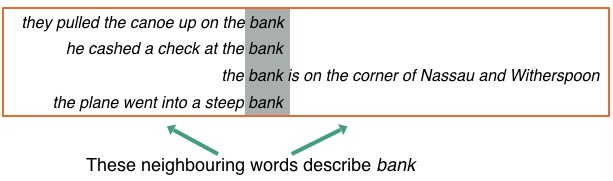
\includegraphics[width=1.0\textwidth]{neighbouring_words} 
	
\end{minipage}%
\label{fig:neighbouring_words}
\caption{Neigboring words defining the specific sense of "bank".}
\end{figure}	
A traditional approach to derive word embeddings is the analysis of the  word co-occurrence matrix \citep{DeerwesterDumaisEtAl1990}. It is based on the one-hot representation. Each row of the matrix represents the information of one word's context, which is sparse and huge. This matrix is decomposed using  singular value decomposition (SVD) to generate low-dimension embedding vectors. The context can be the occurrences of words in the corresponding document  or be the average occurrence's of surrounding words from all documents\com{I do not understand that}. 


Recently, artificial neural networks became very popular to generate lower-dimensional word embeddings. Prominent algorithms are \emph{Senna} \citep{CollobertWeston2008}, \emph{Word2vec} \citep{MikolovSutskeverEtAl2013} and Glove \citep{PenningtonSocherEtAl2014}. They all use randomly initialized vectors to represent words . Subsequently these embeddings are modified in such a way that the word embeddings of the neigboring words may be predicted with minimal error by a simple neural network function. 

\section{Polysemy}

Note that in the approaches described above each word is mapped to a single embedding vector. It is well known, however, that a word may have several different meanings, i.e. is \emph{polysemous}. For example the word "bank" among others may designate: 
\begin{itemize}
	\item the slope beside a body of water,
	\item a financial institution,
	\item a flight maneuver of an airplane.
\end{itemize}
Further examples of polysemy are the words "book", "milk" or "crane".
WordNet \citep{Fellbaum1998} and other lexical resources show, that most common words have 3 to 10 different meanings.
 Obviously each of these meanings should be represented by a separate embedding vector, otherwise the embedding will no longer represent the underlying sense. This in addition will harm the performance of subsequent text mining analyses. Therefore we need methods to learn  embeddings for senses rather than words.


\emph{Sense embeddings} are a refinement of word embeddings. For example, "bank" can appear either together with "money", "account", "check" or in the context of "river", "water", "canoe". And the embeddings of "money", "account", "check" will be quite different from the embeddings of "river", "water", "canoe". Consider the following two sentences 
\begin{itemize}
	\item They pulled the canoe up the bank.
	\item He cashed a check at the bank.
\end{itemize}
The word "bank" in the first sentence has a different sense than the word "bank" in the second sentence. Obviously, the context is different. 
So if we have a methods to determine the difference of the context, we can relabel the word "bank" to the word senses "bank$_1$" or "bank$_2$" denoting the slope near a river or the financial institution respectively. We call the number after the word the sense labels of the word "bank". This process can be performed iteratively for each word in the corpus by evaluating its context.

\com{An alternative representation of words is generated by topic models \citep{BleiNgEtAl2003}, which represent each word of a document as a finite mixture of topic vectors. The mixture weights of a word depend on the actual document. This implies that a word gets different representations depending on the context. Please elaborate}

In the last years a number of approaches to derive sense embeddings have been presented. \cite{HuangSocherEtAl2012} used the clustering of precomputed one-sense word embeddings and their neighborhood embeddings to define the different word senses. The resulting word senses are fixed to the corresponding word neighborhoods and their values are trained until convergence. A similar approach is described by \cite{ChenLiuEtAl2014}. Instead of a single embedding each word is represented by a number of different sense embeddings. During each iteration of the supervised training of Senna or Word2vec for each position of the word the best fitting embedding is selected according the fitness criterion\com{Please reformulate sentence}. Subsequently only this embedding is trained using back-propagation. Note that during training a word may be assigned to different senses thus reflecting the training process. A related approach was proposed by \cite{TianDaiEtAl2014}.

It turned out that the resulting embeddings get better with the size of the training corpus and an increase of the dimension of the embedding vectors. This usually requires a parallel environment for the execution of the training of the embeddings. Recently \emph{Apache Spark} \citep{ZahariaChowdhuryEtAl2010} has been presented, an opensource cluster computing framework. Spark provides the facility to utilize entire clusters with implicit data parallelism and fault-tolerance against resource problems, e.g. memory shortage. The currently available sense embedding approaches are not ready to use compute clusters, e.g. by Apache Spark. 

\section{Goal and Organization of the Thesis}

The main aim of this thesis is to derive expressive word representations for different senses in an efficient way. We will investigate sense assignment models which will extend known word embedding (one sense) approaches. Our goal is to implement such a method on a compute cluster using Apache Spark to be able to process larger training corpora and employ higher-dimensional sense embedding vectors.
\del{Our goal is not to introduce a very excellent method which can get the best sense embedding results, but to try the new model structure like sense assignment and the new software tool like distributed framework Spark to get the results reasonable and efficient.} 
Our main work will focus on the extension of Skip-gram model \citep{MikolovSutskeverEtAl2013} in connection to the approach of \citep{NeelakantanShankarEtAl2015} because these models are easy to use, very efficient and convenient to train. \del{And these days, some JVM based big data frameworks like Apache Spark are more and more popular, but the relative works on neural language processing especially word embedding and sense embedding use very few about these new techniques. That's the main reason that we try to use this new technique to implement our model.} When using the Spark big data framework, we want to gain some experience and get  feedback about the advantages and disadvantages of the new techniques.

\com{Rewrite this if the chapters are finished!}
In the next chapter, we will introduce relative word embedding methods and sense embedding methods. We start with the neural language model and explain the early models of word embeddings. And then we focus on the word2vec \cite{MikolovSutskeverEtAl2013} especially about Skip-gram model. There will be many mathematical details including gradient calculation. After that, we will introduce two famous sense embedding models based the above word embedding works. 
The chapter 3 is our model description for sense embeddings. We use the spark framework to implement our model. The chapter 4 will introduce our implementation and show the experiment we did including parameter comparison and word senses visualization. At last chapter conclusion, we will analysis the advantages and disadvantages about our methods including model and implementation and give some ideas about how we can improve it in the future and what else we can do.



\chapter{Background and Related Works}
\label{cha:embed}

\section{Neural Probabilistic Language Model} 
This section will introduce a neural probabilistic language model from \citep{bengio2003neural}. Such model use a very important tool---Word Embedding. So what is the word embedding? General speaking, for any word $w$ in the dictionary $D$, one can specify a fixed length of real-valued vector $v(w)\in \mathbb{R}^m$, $v(w)$ called the word embedding of $w$, and $m$ is the length of word embedding. A further understanding about the word embeddings will be explained in the next section. 

Since it is a neural probabilistic language model, it is obvious to use an neural network. Figure \ref{fig:neural4} shows the structure of the neural network, it include 4 layers: \textbf{Input} layer, \textbf{Projection} layer, \textbf{Hidden} layer and the \text{Output} layer. $W$ and $U$ are respectively the weight matrix between projection layer and hidden layer and the weight matrix between hidden layer and output layer, \textbf{p} and \textbf{q} are the offset vectors of respectively the hidden layer and the output layer.
 
\begin{figure}[!ht]
  \centering
	\fbox{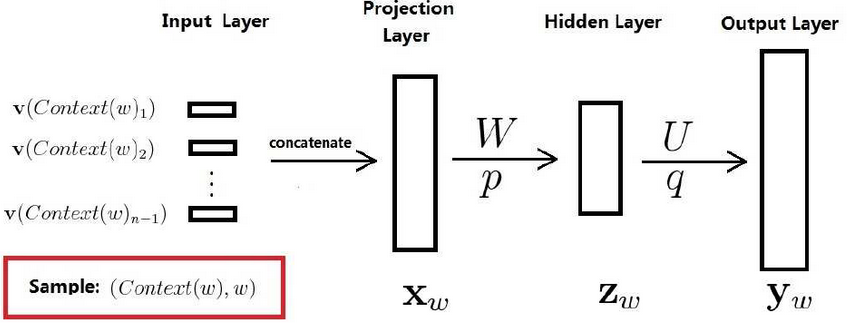
\includegraphics[width=0.7\textwidth]{neural4} }
	\caption{An example of 4 layers neural network}
	\label{fig:neural4}
\end{figure}
 
When talking about the above neural network, generally we consider it as a three-layer structure as following Figure \ref{fig:neural3}. But this thesis still use the structure of Figure \ref{fig:neural4}. On the one hand it is easy to describe, on the other hand it is more convenient to do comparison with the network structure in word2vec.

\begin{figure}[!ht]
  \centering
	\fbox{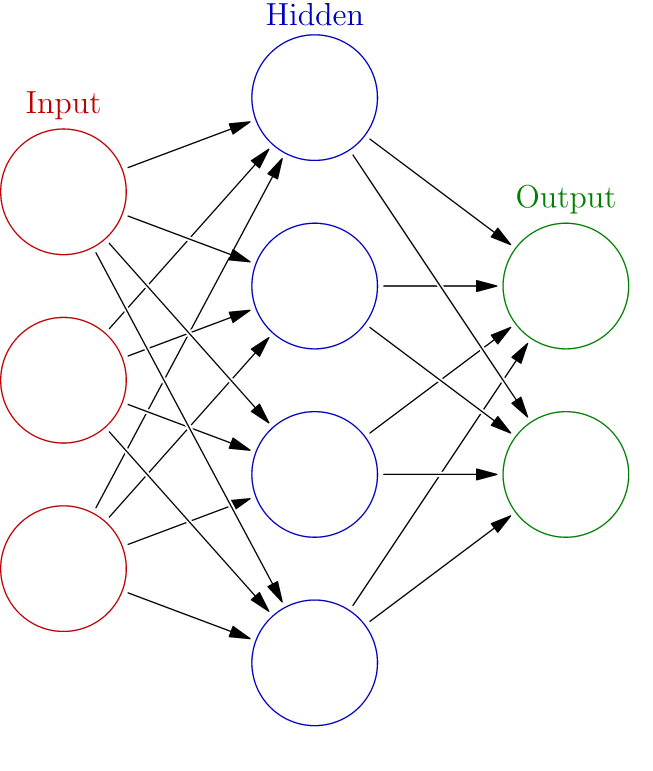
\includegraphics[width=0.5\textwidth]{neural3} }
	\caption{An example of 3 layers neural network}
	\label{fig:neural3}
\end{figure}

\citep{bengio2003neural} also considers the connection of some neurons from projection layer and some neurons from hidden layer as Figure \ref{fig:bengio}. Thus, there is one more weight matrix. In the numerical experiments, the author found that the introduction of the weight matrix projection layer and output layer can not improve the model effect, but it can reduce the number of training iterations.\\

\begin{figure}[!ht]
  \centering
	\fbox{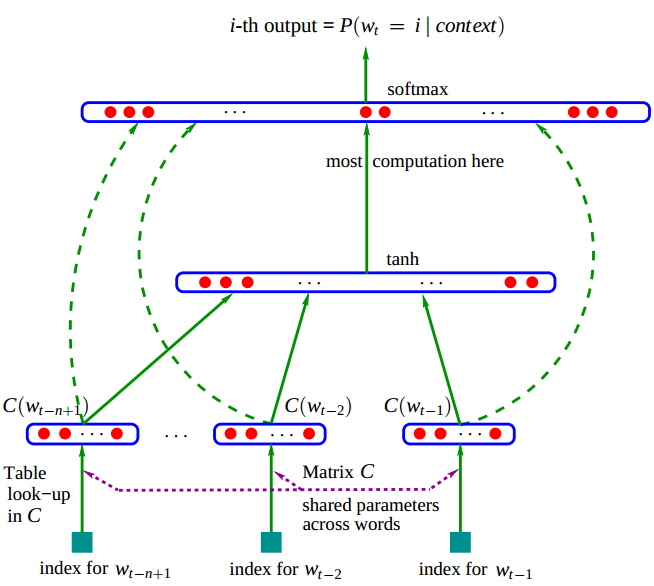
\includegraphics[width=0.7\textwidth]{bengio} }
	\caption{The neural network structure from \citep{bengio2003neural}}
	\label{fig:bengio}
\end{figure}

For any word $w$ in corpus $C$ , assuming $Context(w)$ takes its front $n-1$ words (similar to the n-gram), this binary pair $(Context (w), w)$ is a a training sample. So how is the sample $(Context (w), w)$ involved in computing through the neural network? Note that once word corpus $C$ and vector length $m$ is given, the scale of projection layer and the scale of output layer are determined. The former is $(n-1)m$, the latter is $N=|D|$, that is, the size of vocabulary. The size of the hidden layer $n_h$ is the adjustable parameter which can be specified by the user.

Why is the size of the projected layer $(n-1)m$? In fact, the input layer includes $n-1$ words from $Context(w)$, and the vector $\mathbf{x_w}$ from projected layer is built: concatenate $n-1$ input word vectors to be a long vector whose length is $(n-1)m$. With the vector $\mathbf{x_w}$ , the next calculation is clear
\begin{equation}\label{eq:neural4}
\left\{
\begin{aligned}
\mathbf{z_w} & =  \tanh(W x_w+\mathbf{p}),\\
\mathbf{y_w} & =  U z_w + \mathbf{q}\\
\end{aligned}
\right.
\end{equation}
where $\tanh$ is the Hyperbolic Tangent Function, used as the Active Function in the hidden layer. In the above formula, $\tanh$ acting on the vector represents acting each component of the vector. How about the number of first few words of a given sentence is less than $n-1$? Usually, we can artificially add some filler vectors, and they will also be involved in the training process.\\

From the above two steps, we get $\mathbf{y_w}=(y_{w,1},y_{w,2},\ldots,y_{w,N})^T$, which is just the vector with the length of $N$ and its components can not represent probabilities. If you want to use $\mathbf{y_w}$'s component $y_ {w,i}$ to represent that the probability of the next word is the $i$-th word when the context is $Context(w)$. Also you need to do a softmax normalization. After normalization, $p(w|Context(w))$ can be expressed as
\begin{equation}\label{eq:softmax}
p(w|Context(w))=\frac{e^{y_{w,i_w}}}{\sum^N_{i=1}e^{y_{w,i}}},
\end{equation}
where $i_w$ represents the index of $w$ in the dictionary $D$.

Formula \ref{eq:softmax} gives the function representation of the probability $p(w|Context(w))$, that is, it gives the function mentioned in the last section $F(w,Context(w),\theta)$. So what is the $\theta$? In conclusion, there are two parts \\
\begin{itemize}
\item Word vectors: $\mathbf{v}(w)\in \mathbb{R}^m, w\in D$ and the filter vectors
\item Neural network parameters: $W\in \mathbb{R}^{n_h*(n-1)m}, \mathbf{p}\in \mathbb{R}^{n_h}; U \in \mathbb{R}^{N*n_h}, \mathbf{q}\in \mathbb{R}^N$
\end{itemize}
These parameters can be obtained by the training algorithm. On thing needs to be mentioned that, in common machine learning algorithms, the input is already known, however in the above neural probability language model shown as Figure \ref{fig:neural4}, the input $\mathbf{v}(w)$ is not known and also needs to be training.

The next, let's loot at the computation of the above model. In the above neural network, the scales of the projection layer, the hidden layer and the output layer are respectively $(n-1)m$, $n_h$, $N$, let's look at the parameters involved:
\begin{enumerate}
\item $n$ is the number of words contained in the context of a word, usually no more than 5
\item $m$ is the length of word vector, usually the magnitude of $10^1\sim10^2$
\item $n_h$ is specified by the customer, usually not too big, like the magnitude of $10^2$
\item $N$ is the size of corpus vocabulary , related with the corpus, usually the magnitude of $10^4\sim10^5$  
\end{enumerate}
Recombination with \ref{eq:neural4} and \ref{eq:softmax}, it is not difficult to find that, the computing of entire model is mainly about the matrix-vector operations between the hidden layer and the output layer and the softmax normalization in the output layer. Therefore, many of subsequent related works are about optimization for this part, including the the work of word2vec. 

Comparison with n-gram model, neural probabilistic language model mainly has the following two advantages:

\begin{enumerate}
\item Similarity between words can be be reflected in the word vectors.

\tab If in an (English) corpus, $S_1$ = \lq\lq A dog is running in the room\rq\rq\ appears 10000 times, and $S_2$ = \lq\lq A cat is running in the room\rq\rq\ only appears once. According to the n-gram model, $p(S_1)$ will certainly be much greater than $p(S_2)$. Note that the only difference between $S_1$ and $S_2$ is the \lq\lq dog\rq\rq\ and \lq\lq cat\rq\rq\ , but this two words play the same role either semantically or grammatically, so $p(S_1)$ and $p(S_2)$ should be very close.

\tab However, the probabilities $p(S_1)$ and $p(S_2)$ calculated by the neural network are approximately equal. The reason is that: 
\begin{enumerate}
\item In the neural network probabilistic language model, there is an assumption that the \lq\lq similar \rq\rq\ words should have similar vectors
\item The probability function on the word vectors is smooth, that is there is only very small influence for the probability when word vector change a little. 
\end{enumerate}
As a result, for the following sentences
\begin{labeling}{alligator}
\item [\tab A dog is running in the room] 
\item [\tab A cat is running in the room]
\item [\tab The cat is running in a room] 
\item [\tab A dog is walking in a bedroom] 
\item [\tab The dog was walking in the room] 
\item [\tab \tab ...] 
\end{labeling}
anyone appears in the corpus, the probabilities of other sentences will increase accordingly.
\item Models based on the word vector have smoothing already (from \ref{eq:softmax}, we can know $p(w|Context(w))\in(0,1)$ can not be $0$), no longer need to carry the additional processing like n-gram model.
\end{enumerate}

Finally, let's look back and think about what kind of role the word vector plays in the neural probability model. When training, it is just the auxiliary parameter used to construct the objective function; after the training, it seems just a by-product of the language model. However, this by-product can not be underestimated, the next section will be further elaborate its usefulness.
%--------------------------------------------------------------------------------------------------------------------------------%
\section{Understanding of the Word Embedding}
In NLP tasks, we will use machine learning algorithms to deal with natural language, but the machine can not directly understand human language, so the first thing is to transform the language to the mathematical form. How can we do such thing? Word vector provides a solution.\\

One of the easiest word vector is one-hot representation, which is to use a long vector to represent a word, the vector's length is  $N$, the size of dictionary $D$. It only has one component which is 1, and the other components are all 0s. The position of 1 corresponds to the index of the word in dictionary. But this word vector representation has some disadvantages, such as troubled by the huge dimensionality, especially when it is applied to deep learning scenes; another thing, it can not describe the similarity between words very well. Another word vector is Distributed Representation, it was firstly proposed by \cite{williams1986learning}, which can overcome the above drawbacks from one-hot representation. The basic idea is to train the particular language to map each word into a short vector of fixed length (here \lq\lq short\rq\rq\ is respected to \lq\lq long\rq\rq\ in one-hot representation). All of these vectors constitute a vector space, and each can be regarded as a a point in the vector space. After introducing the \lq\lq distance\rq\rq in this space , it is possible to judge the similarity between words (morphology and syntax) according to the distance. Actually, word2vec uses this Distributed Representation for word vector.\\

Why is it called Distributed Representation? For one-hot representation, there is only one non-zero vector component, which is very concentrated. For Distributed Representation, vectors have a lot of non-zero components, relatively dispersed. It distributes the information of the word into each component, which is very similar as distributed parallel.\\

Suppose that there are $a$ different points distributed on the two-dimensional plane, giving a point from them, the task is to find another point closest to this point in the plane. How can we do it? Firstly, establish a Cartesian coordinate system. Based on this coordinate system, each point on which uniquely corresponds to a coordinate $(x, y)$; and then introduce the Euclidean distance; finally calculate the distance between this point and other $a-1$ points, from which the point with the minimum distance is the one we are looking for. In the above example, the role of the coordinates $(x, y)$ is equivalent to the word vector. It is used to mathematically quantify a point on a plane. After the coordinate system is set up, it is very easy to get the coordinate of a point. However, for NLP tasks, to get the word vector is more complex, and the word vector is not unique, which depends on the quality of the training data, training algorithm and other factors.\\

A good word vector is valuable, for example, Ronan Collobert's team makes use of the word vector from software package SENNA (\citep{collobert2011natural}) to do POS, CHK, NER and other tasks, and achieves good results. Google's Tomas Mikolov team has developed an automatic generation technology for dictionary and glossary, which is able to convert one language into another language. The relation collection between words in each language, that is \lq\lq language space\rq\rq\ , can be characterized as a set of vectors in the mathematical sense.  As long as the mapping and translation of a vector space to another vector space are realized, language translation can be realized. This technique has very good performance for translation between English and Spanish, with the accuracy rate up to $90\%$. 

\section{C$\&$W's Model}

C$\&$W's original main purpose is not to generate a good word vectors, or even do not want to train the language model, but to use this word vectors to complete several tasks from natural language processing, such as speech tagging, named entity recognition, phrase recognition, semantic role labeling, and so on (\citep{collobert2008unified} and \citep{collobert2011natural}). Due to the different purpose, their training method is also different and special. They do not use language model's idea like optimizing the probability $P( w_t| w_1, w_2, ... , w_{t - 1})$, but directly use the score $f( w_{t - n + 1}, ... , w_{t - 1}, w_t)$ to determine if the sentence is reasonable and normal; low score illustrates the sentence is not reasonable; if you put a few words randomly together, it would be certainly a negative score. The score is just about high or low, not business with probabilities. 

With the above assumption, C$\&$W used the pair-wise method to train the word vectors. Specifically, it is to minimize the following objective function.

$$\sum_{x\in X}\sum_{w\in D}max\{0,1-f(x),f(x^{(w)})\}$$

$X$ is the set of all consecutive $n$-length phrases, D is the entire dictionary. The first summation enumerates all $n$-length phrases from the training set, and each of them positive sample. The second summation for dictionary is to build negative samples. $x(w)$ means the phrase $x$ replacing the middle word to the word $w$. In most cases, replacing the middle of the word in a normal phrase, the new phrase is certainly not the normal phrase, which is a good method to build negative sample (in most cases they are negative samples, only in rare cases the normal phrases are considered as negative samples but they would not affect the final result). \\

The structure of $f$ is almost save as the network structure from \citep{bengio2003neural}. The same thing is connecting $n$ word vectors together to get a long vector and passing through one layer (a matrix multiplication) to get the hidden layer. The difference is that C$\&$W's output layer has only one node representing the score, rather than Bengio's $|V|$ nodes. Doing so greatly reduced the computational complexity. Of course, C$\&$W does not want to make a real language model, but just use some idea from the language model to assist them to complete other tasks in NLP. 

Specifically, they give two different neural network structures window approach and sentence approach, shown as Figure \ref{fig:cw1} and Figure \ref{fig:cw2} respectively. Window approach is a feedforward neural network including a linear layer, HardTanh layer. Its input is the the vector concatenated by all all word vectors within the current word window including itself. Window approach is able to deal with most of natural language processing tasks, but has very poor performance on SRL taks. There, they proposed sentence approach to solve such problem. It is convolutional neural network structure. Apart from the linear layer and HardTanh layer, it has another convolutional layer and Max layer. 

\begin{figure}[H]
\centering
\begin{minipage}{.5\textwidth}
 
	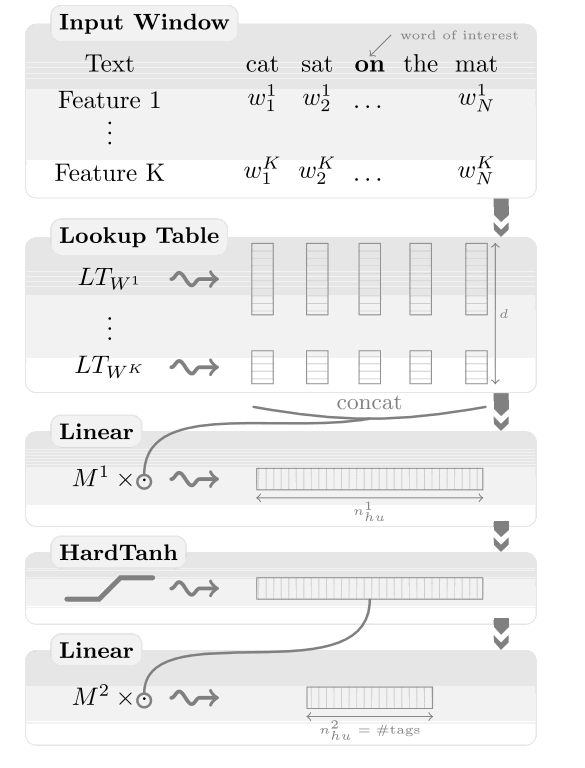
\includegraphics[width=0.9\textwidth]{cw1} 
	\caption{window approach(\cite{collobert2011natural})}
	\label{fig:cw1}
\end{minipage}%
\begin{minipage}{.5\textwidth}
  
	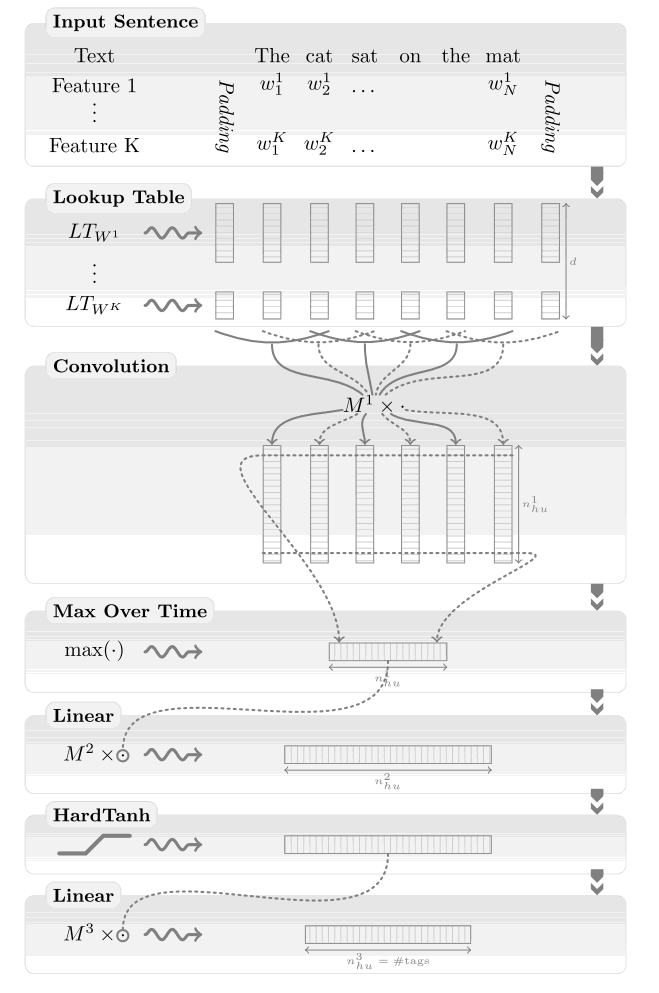
\includegraphics[width=0.85\textwidth]{cw2}
	\caption{sentence approach (\citep{collobert2011natural})}
	\label{fig:cw2}
\end{minipage}
\end{figure}

In the experiment the size of window $n$ is 11 and the size of dictionary $|V|$ is 130000. They spent totally seven weeks to train word vectors from the Wikipedia English corpus and Reuters corpus.

\section{Word2Vec}
This section will introduce two important model in word2vec: CBOW model (Continuous Bag-of-Words Model) and Skip-gram model (Continuous Skip-gram Model). 

From the figure, two models both include three layers: \textbf{Input Layer}, \textbf{Projection Layer}, \textbf{Output Layer}. The former is to predict the current word $w_t$ giving its context $w_{t-2}$,$w_{t-1}$,$w_{t+1}$,$w_{t+2}$

With the foregoing preparation, this section describes word2vec officially used in two important models --CBOW model (Coutinuous Bag-of-Words Model) and Skip-gram model (Continuous Skip-gram Model). About two models, \cite{mikolov2013distributed} shows the schematic diagram shown in Figures \ref{fig:CBOW} and \ref{fig:Skip-Gram}.
Be seen by the two models contain three layers: \textbf{Input layer}, \textbf{projection layer}  and \textbf{output layer}. The former is known in the current word $w_t$ context $w_{t-2}$, $w_{t-1}$, $w_{t+1}$, $w_{t+2}$ premise predictive current word $w_t$ (see Figure 8); and the latter on the contrary, it is known in the current word $w_t$ premise predict its context $w_{t-2}$, $w_{t-1}$ , $w_{t+1}$, $w_{t+2}$ (see Figure 9).
For two CBOW and Skip-gram model, word2vec given two frameworks, which are based on Hierarchical Softmax and Negative Sampling to design. This section describes the Hierarchical Softmax CBOW and Skip-gram model.
In the previous section, we mentioned that the objective function neural network based language model is generally taken as follows log-likelihood function
$$\mathcal{L}=\sum_{w\in\mathcal{C}}\mathrm{log}\ p(w|Context(w)), $$
The key is the conditional probability function $p(w|Context(w))$ configuration, text [] in this model is given a construction method function (see (3.6) formula).
For the objective function Hierarchical Softmax CBOW word2vec model based on optimized also the form (4.1); and for the objective function based on Hierarchical Softmax of Skip-gram model, the optimization of the form
$$\mathcal{L}=\sum_{w\in\mathcal{C}}\mathrm{log}\ p(Context(w)|w), $$
Therefore, the discussion process, we should focus on the $p(w|Context(w))$ or $p(Context(w)|w)$ on the structure, realize that this is very important because it allows us to targeted, distractions, and will not fall into some of the tedious details were to go. Next, we will focus on the Skip-gram model with negative sampling and explain some mathematical details, because our model is based that.

\begin{center}
\begin{figure}[H]
\centering
\begin{minipage}{.5\textwidth}
 
	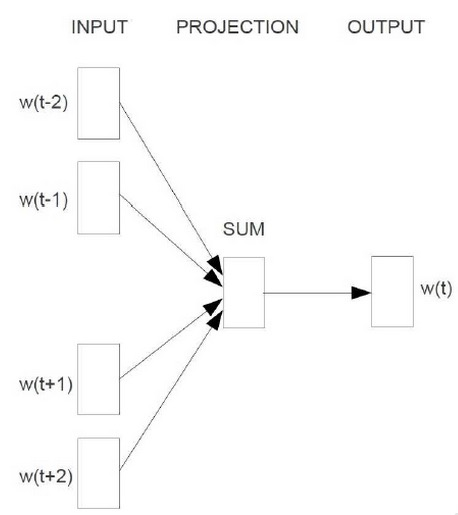
\includegraphics[width=0.9\textwidth]{CBOW} 
	\caption{CBOW model}
	\label{fig:CBOW}
\end{minipage}%
\begin{minipage}{.5\textwidth}
  
	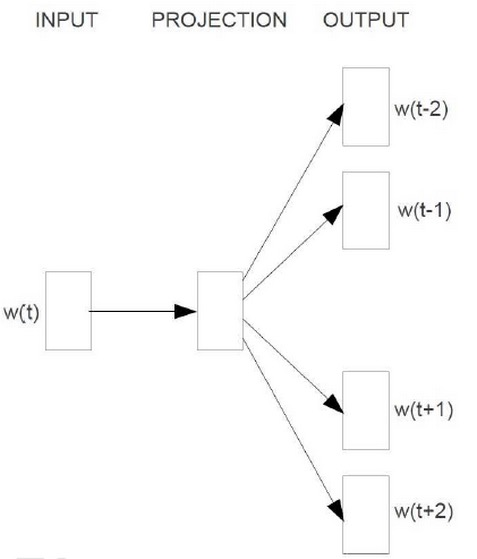
\includegraphics[width=0.85\textwidth]{Skip-Gram}
	\caption{Skip-Gram model}
	\label{fig:Skip-Gram}
\end{minipage}
\end{figure}
\end{center}

\subsection{Skip-gram model with Hierarchical Softmax}
This section describes word2vec another model -- Skip-gram model, since the derivation and CBOW similar, and therefore will inherit the measure introduced mark.

Figure 12 shows the network structure of Skip-gram model, with network structure CBOW model, it also includes three layers: an input layer, a projection layer and output layer. The following sample $(w,Context(w))$, for example, three layers are described briefly.
\begin{enumerate}
\item \textbf{input layer}: the center of the current sample containing only the word $w$ word vector $\mathbf{v}(w)\in\mathbb{R}^m$.
\item \textbf{projection layer}: This projection is identical to $\mathbf{v}(w)$ projection to $\mathbf{v}(w)$. Therefore, this projection layer is actually superfluous reason here mainly to facilitate retention projection layer and network structure CBOW models do comparison.
\item \textbf{Output layer}: and CBOW model, the output layer is also a lesson Huffman tree.
\end{enumerate}
\subsubsection {Gradient Calculation} 
For Skip-gram model, it is known that the current word $w$, need to predict its context $Context(w)$ of the words, the objective function should therefore form (4.2), and the key is the conditional probability function $p(Context(w)|w)$ configuration, in the Skip-gram model which is defined as
$$p(Context(w)|w)=\prod_{u\in Context(w)}^{p(u|w},$$
In the above formula $p(u|w)$ in accordance with section describes the Hierarchical Softmax thought, similar to (4.3) written as
$$p(u|w)=\prod_{j = 2}^{l^u}p(d^u_j|\text{v}(w),\theta^u_{j-1}), $$
among them
\begin{equation}
p(d^u_j|\mathbf{v}(w),\theta^u_{j-1})=[\theta(\mathbf{v}(w)^{\mathrm{T}}\theta^u_{j-1})]^{1-d^u_j}\cdot[1-\theta(\mathbf{v}(w)^{\mathrm{T}}\theta^u_{j-1})]^{1-d^u_j}
\end{equation}
The (4.6) followed by generations back, you can get the log-likelihood function (4.2) of the specific expression
\begin{equation}
\mathcal{L}=\sum_{w\in\mathcal{C}}\mathrm{log}\prod_{u\in Context(w)}\prod_{j=2}^{l^u}\{[\theta(\mathbf{v}(w)^{\mathrm{T}}\theta^u_{j-1})]^{1-d^u_j}\cdot[1-\theta(\mathbf{v}(w)^{\mathrm{T}}\theta^u_{j-1})]^{\ d^u_j}\} \\
\ \ \ $$ $$=\sum_{w\in\mathcal{C}}\sum_{u\in Context(w)}\sum_{j=2}^{l^u}\{(1-d^u_j)\cdot\mathrm{log}[\theta(\mathbf{v}(w)^{\mathrm{T}}\theta^u_{j-1})]+d^u_j\cdot\mathrm{log}[1-\theta(\mathbf {v}(w)^{\mathrm{T}}\theta^u_{j-1})]\}.
\end{equation}
Similarly, as in the following gradients of convenience, under the triple summation symbol braces contents of abbreviated as $\mathcal{L}(w,u,j)$, ie
$$\mathcal{L}(w,u,j)=(1-d^u_j)\cdot\mathrm{log}[\theta(\mathbf{v}(w)^{\mathrm{T}}\theta^u_{j-1})]+d^u_j\cdot\mathrm{log}[1-\theta(\mathbf{v}(w)^{\mathrm{T}}\theta^u_{j-1}]. $$
So far, it has been deduced logarithmic likelihood function of expressions like (4.7), which is the objective function Skip-gram model. Then also use stochastic gradient ascent method to optimize the key is to give two types of gradients.
First consider $\mathcal{L}(w,u,j)$ on $\theta^u_{j-1}$ gradient calculation (with the corresponding portion of the model is derived CBOW completely analogous).
$$\partial\frac{\mathcal{L}(w, u, j)}{\partial\theta^u_{j-1}}=\frac{\partial}{\partial\theta^u_{j-1}}\{(1-d^u_j)\cdot\mathrm{log}[\theta(\mathbf{v}(w)^{\mathrm{T}}\theta^u_{j-1})]+d^u_j\cdot\mathrm{log}[\theta(\mathbf{v}(w)^{\mathrm{T}}\theta^u_{j-1})]\}$$

\subsection{Skip-gram with Negative Sampling}

Negative Sampling (NEG) is proposed by Tomas Mikolov et al.[word2vec]  , which is the simplified version of NCE(Noise Contrastive Estimation), the purpose is to improve the training and the quality of word vectors. Comparison with Hierarchical Softmax, NEG do not use the Huffman tree. Instead, it use Random Negative Sampling, which can improve the performance much.

The details of NCE is a little complex, the essence is to use a known probability density function to estimate an unknown probability density function. In short, assume there is an unknown probability density function $Y$ and a known probability density function $X$, if we get the relationship between $X$ and $Y$, we can obtain $X$ as well.The detail of method reference to [NCE]. 

The objective function is:
\begin{equation}
G=\prod_{w\in\mathcal{C}}\prod_{u\in Context(w)}g(u),
\end{equation}
Here, we want to maximize $\prod_{u\in Context(w)}g(u)$ giving $(w, Context(w)))$,  and $g(u)$ is defined as
$$g(u)=\prod_{z\in{u}\cup NEG(u)}p(z|w),$$
where $NEG(u)$ represents the negative samples generated by $u$, the conditional probability
$$p(z|w)=\left\{
\begin{aligned}
\sigma(\mathbf{v}(w)^{\mathrm{T}}\theta^z), && L^u(z)=1; \\
1-\sigma(\mathbf{v}(w)^{\mathrm{T}}\theta^z), && L^u(z)=0; \\
\end{aligned}
\right.
$$
where $$L^u(z) = \left\{
\begin{aligned}
1, && u = z;\\
0, && u \neq z,\\
\end{aligned}
\right.
$$
It can also be written as one expression
\begin{equation}
p(z|w)=[\sigma(\mathbf{v}(w)^{\mathrm{T}}\theta^z)]^{L^u(z)}\cdot[1-\sigma(\mathbf{v}(w)^{\mathrm{T}}\theta^z)]^{1-L^u(z)}
\end{equation}
And then we use the log of $G$, so the final objective function is 
\begin{align*}
L & =\mathrm{log}\ G=\mathrm{log} \prod_{w\in\mathcal{C}}\prod_{u\in Context(w)} g(u)=\sum_{w\in\mathcal{C}}\sum_{u\in Context(w)} \mathrm{log}\ g(u) \\
& = \sum_{w\in\mathcal{C}}\sum_{u\in Context(w)} \mathrm{log} \prod_{z\in\{u\}\cup NEG(u)} p(z|w) \\
& = \sum_{w\in\mathcal{C}}\sum_{u\in Context(w)}\sum_{z\in\{u\}\cup NEG(u)} \mathrm{log}\ p(z|w) \\
& = \sum_{w\in\mathcal{C}}\sum_{u\in Context(w)}\sum_{z\in\{u\}\cup NEG(u)} \mathrm{log}\ \{[\sigma(\mathbf{v}(w)^{\mathrm{T}}\theta^z)]^{L^u(z)}\cdot[1-\sigma(\mathbf{v}(w)^{\mathrm{T}}\theta^z)]^{1-L^u(z)}\} \\
& = \sum_{w\in\mathcal{C}}\sum_{u\in Context(w)}\sum_{z\in\{u\}\cup NEG(u)}\{L^u(z)\cdot \mathrm{log}[\sigma(\mathbf{v}(w)^{\mathrm{T}}\theta^z)]+[1-L^u(z)]\cdot\mathrm{log}[1-\sigma(\mathbf{v}(w)^{\mathrm{T}}\theta^z)]\}.
\end{align*}
In order to calculate the gradient more conveniently, we use $L(w,u,z)$ to represent the contents of curly braces as
$$\mathcal{L}(w,u,z)=L^u(z)\cdot \mathrm{log}[\sigma(\mathbf{v}(w)^{\mathrm{T}}\theta^z)]+[1-L^u(z)]\cdot\mathrm{log}[1-\sigma(\mathbf{v}(w)^{\mathrm{T}}\theta^z)]$$
And next, let's use \textbf{Stochastic gradient ascent method} to optimize it. The point is to calculate two kinds of gradient. Let's consider the gradient $\theta^z$ firstly.
\begin{align*}
& \ \ \ \ \frac{\partial\mathcal{L}(w,u,z)}{\partial\theta^z} \\
& =  \frac{\partial}{\partial\theta^z} \{ L^u(z)\cdot \mathrm{log}[\sigma(\mathbf{v}(w)^{\mathrm{T}}\theta^z)]+[1-L^u(z)]\cdot\mathrm{log}[1-\sigma(\mathbf{v}(w)^{\mathrm{T}}\theta^z)] \} \\
& =  L^u(z)[1-\sigma(\mathbf{v}(w)^{\mathrm{T}}\theta^z)]\mathbf{v}(w) - [1-L^u(z)]\sigma(\mathbf{v}(w)^{\mathrm{T}}\theta^z)\mathbf{v}(w) \\
& = \{L^u(z)[1-\sigma(\mathbf{v}(w)^{\mathrm{T}}\theta^z)]-[1-L^u(z)]\sigma(\mathbf{v}(w)^{\mathrm{T}}\theta^z)\}\mathbf{v}(w) \\
& = [L^u(z)-\sigma(\mathbf{v}(w)^{\mathrm{T}}\theta^z)] \mathbf{v}(w).
\end{align*}
Thus, the updating formula of $\theta^z$ can be written as
$$\theta^z:=\theta^z+\eta[L^u(z)-\sigma(\mathbf{v}(w)^{\mathrm{T}}\theta^z)]\mathbf{v}(w).$$
The next, let's consider the gradient of $\mathbf{v}(w)$. Using the symmetry of \textbf{v}(w) and $\theta^z$, we have
$$\frac{\partial\mathcal{L}(w,u,z)}{\partial\mathbf{v}(w)} = [L^u(z)-\sigma(\mathbf{v}(w)^{\mathrm{T}}\theta^z)]\theta^z,$$
Thus, the updating formula of $\mathbf{v}(u)$ can be written as 
$$\mathbf{v}(w):=\mathbf{v}(w)+\eta\sum_{z\in\{u\}\cup NEG\{u\}}\frac{\partial\mathcal{L}(w,u,z)}{\partial\mathbf{v}(w)}$$
$$=\mathbf{v}(w)+\eta\sum_{z\in\{u\}\cup NEG\{u\}}[L^u(z)-\sigma(\mathbf{v}(w)^{\mathrm{T}}\theta^z)]\theta^z.$$

\section{Huang's Model}


Eric H. Huang's work (\cite{huang2012improving}) is based on the model from \cite{collobert2008unified}. The goal of his working is about trying to make the word vectors with richer semantic information than other models. He had two major innovations to accomplish this goal : The first innovation is using global information from the whole text to assist local information, the second innovation is using the multiple word vectors to represent polysemy. \\

Huang thinks C$\&$W's work uses only "local context". In the process of training vectors, C$\&$W used only 10 words as the context for each word, counting the center word itself, there are totally 11 words' information. 
These local information can not fully exploit the semantic information of the center word. Huang used C$\&$W's neural network directly to compute a score as the "local score". 
And then Huang proposed a "global information", which is somewhat similar to the traditional bag of words model. Bag of words is about accumulating One-hot Representation from all the words of the article together to form a vector (like all the words thrown in a bag), which is used to represent the article. Huang's global information used the average weighted vectors from all words in the article (weight is word's idf), which is considered the semantic of the article. 
He connected such semantic vector of the article (global information) 
with the current word's vector (local information) to form a new vector with double size as an input, and then used the C$\&$W's network to calculate the score. Figure [huang] shows such structure.
With the "local score" from original C$\&$W approach and "Global score" from improving method based on the C$\&$W approach, Huang directly add two scores as the final score. The final score would be optimized by the pair-wise target function from C$\&$W. Huang found his model can capture better semantic information. \\

\begin{figure}[!ht]
  \centering
	\fbox{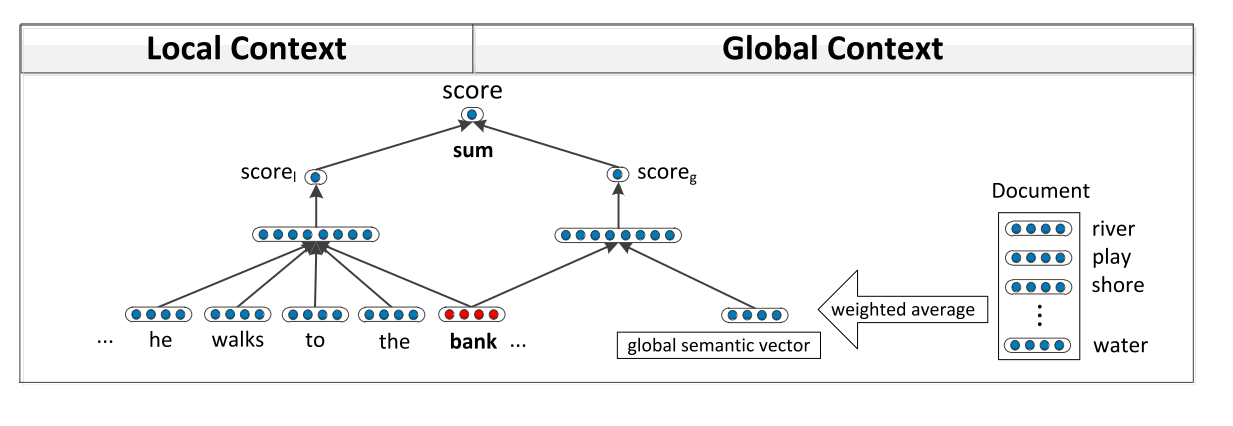
\includegraphics[width=0.9\textwidth]{huang} }
	\caption{The network structure from \citep{huang2012improving}}
	\label{fig:huang}
\end{figure}


The second contribution of this paper is to represent polysemy using multiple word vectors. \citep{bengio2003neural} also mentioned that this would be an very important issue, but he was still looking for a solution, now Huang gives an idea. For each center word, he took 10 nearest context words and calculated the weighted average of these 10 word vectors (idf weights) as the context vector. Huang used all context vectors to do k-means clustering, and relabel  each word based on the clustering results (different classes of the same words would be considered as different words to process), and finally re-trained the word vectors. The following gives some examples from his model's results.\\

\begin{center}

 \begin{tabular}{|l|l|}
  \hline
  Center Word &Nearest Neighbors \\
  \hline  
  bank$\_$1 & corporation, insurance, company\\
  \hline
  bank$\_$2 & shore, coast, direction\\
  \hline
  star$\_$1 & movie, film, radio\\
  \hline
  star$\_$2 & galaxy, planet, moon\\
  \hline
  cell$\_$1 & telephone, smart, phone\\
  \hline
  cell$\_$2 & pathology, molecular, physiology\\
  \hline
  left$\_$1 & close, leave, live\\
  \hline
  left$\_$2 & top, round, right\\
  \hline
 \end{tabular}
\end{center}
\section{EM-Algorithm based method}


There is a very famous method based on the EM-algorithm from \cite{tian2014probabilistic}. This method is the extension of normal skip-gram model. They still use each center word to predict several context words. The difference is that each center word can have several senses with different probabilities. The probability can represent if a sense is used frequent in the corpus. For example, considering $bank_1$ and $bank_2$, $bank_1$ represents the side of the river with the smaller probability and $bank_2$ means the institute about money with the higher probability. We can say in the corpus, in most sentences of the corpus the word "bank" means the institute about money and in other fewer cases it means the side of the river. \\

\paragraph{Objective Function}\ \\

Considering $w_I$ as the input word and $w_O$ as the output word, $(w_I,w_O)$ is a data sample. The input word $w_I$ have $N_{w_I}$ prototypes, and it appears in its $h_{w_I}$-th prototype, i.e., $h_{w_I}\in \{1,..,N_{w_I}\}$ [] The prediction $P(w_O|w_I)$ is like the following formula

$$p(w_O|w_I)=\sum^{N_{w_I}}_{i=1}P(w_O|h_{w_I}=i,w_I)P(h_{w_I}=i|w_I)=\sum^{N_{w_I}}_{i=1}\frac{exp(U^{\mathrm{T}}_{w_O}V_{w_I,i})}{\sum_{w\in W exp(U^\mathrm{T}_w V_{w_I,i})}}P(h_{w_I}=i|w_I)$$

where $V_{w_I,i}\in R^d$ refers to the d-dimensional "input" embedding vector of $w_I$'s $i$-th prototype and $U_{w_O}\in R^d$ represents the "output" embedding vectors of $w_O$. Specifically, they use the Hierarchical Softmax Tree function to approximate the probability calculation. 

\paragraph{Algorithm Description}\ \\

Particularly for the input word $w$, they put all samples ($w$ as the input word) together like $\{(w, w_1), (w, w_2), (w, w_3) ... (w, w_n)\}$ as a group. Each group is based on the input word. So the whole training set can be separated as several groups. For the group mentioned above, one can assume the input word $w$ has $m$ vectors ($m$ senses), each with the probability $p_j (1 \leq j \leq m)$. And each output word $w_i (1 \leq i\leq n)$ has only one vector. \\

 In the training process, for each iteration, they fetch only part of the whole training set and then split it into several groups based on the input word. In each E-step, for the group mentioned above, they used soft label $y_{i,j}$ to represent the probability of input word in sample $(w,w_i)$ assigned to the $j$-th sense. The calculating of $y_{i,j}$ is based on the value of sense probability and sense vectors. After calculating each $y_{i,j}$ in each data group, in the M-step, they use $y_{i,j}$ to update sense probabilities and sense vectors from input word, and the word vectors from output word. The following are some results from this model.


\begin{tabular}{|l|l|l|}
  \hline
  word & Prior Probability & Most Similar Words \\
  \hline  
  apple$\_$1 & 0.82 & strawberry, cherry, blueberry\\
  \hline
  apple$\_$2 & 0.17 & iphone, macintosh, microsoft\\
  \hline
  bank$\_$1 & 0.15 & river, canal, waterway\\
  \hline
  bank$\_$2 & 0.6 & citibank , jpmorgan, bancorp\\
  \hline
  bank$\_$3 & 0.25 & stock, exchange, banking\\
  \hline
  cell$\_$1 & 0.09 & phones cellphones, mobile\\
  \hline
  cell$\_$2 & 0.81 & protein, tissues, lysis\\
  \hline
  cell$\_$3 & 0.01 &locked , escape , handcuffed\\
  \hline
 \end{tabular}

\chapter{Model}
\label{cha:modeli}

Generally speaking, our model is a extension of skip-gram model with negative sampling. We assume each word in the sentence can have one or several senses. But unlike Huang's model (\cite{huang2012improving}), they use clustering results to label word senses and once assigned these senses can not be changed. Our model is different, we do not use any pre work to assign senses (label words), instead we just assign each word with random senses and they can be adjusted afterwards. We also follow the idea from EM-Algorithm based method (\citep{tian2014probabilistic}), word's different senses have different probabilities, the probability can represent if a sense is used frequent in the corpus. \\

In fact, after some experiments, we found our original model is not good. So we simplified our original model. Anyhow we will introduce our original model and show the failures in the next chapter, and explain the simplification. 

\section{Definition}

\ \ \ \ \ \ $C$ is the corpus and $D$ is the vocabulary. We consider that the training corpus $C$ is made up by $M$ sentences, like $(S_1,S_2,\ldots,S_M)$, and each sentence is made up by several words like $S_i = (w_{i,1},w_{i,2},\ldots,w_{i,L_i})$ and $L_i$ is the length of sentence $S_i$. We use $w_{i,j}$ to represent the word token in the position $j$ of sentence $S_i$. Each word in each sentence has one or multiple senses. We use $h$ to lookup table of sense assignment, specifically $h_{i,j}$ is the sense index of word $w_{i,j}$  ($1\leq h_{i,j}\leq N_{w_{i,j}}$), where $N_w$ is the max number of senses of word $w$ ($w\in D$)\\

We use $V$ and $U$ to represent respectively the set of input embedding vectors and the set of output embedding vectors respectively. And each embedding vectors has the dimension $d$. Additionally, $V_{w,s} \in \mathbb{R}^d$ means the input embedding vectors from sense $s$ of word $w$, similarly as the definition of $U_{w,s}$, where  $w\in D$, $1\leq s\leq N_w$. Following the Skip-gram model with negative sampling, $K$ is the number of negative samples and $c$ is the size of context. And $P_n(w)$ is the smoothed unigram distribution which is used to generate negative samples. Specifically, $P_n(w) = \frac{count(w)^{\frac{3}{4}}}{(\sum_{i=1}^M L_i)^{\frac{3}{4}}}$ ($w\in D$), where $count(w)$ is the number of times $w$ occurred in $C$ and $\sum_{i=1}^M L_i$ is the number of total words in $C$.

\section{Objective Function}
\begin{equation}
\begin{split}
G = \frac{1}{M}\sum_{i=1}^M\frac{1}{L_i}\sum_{t=1}^{L_i}\sum\limits_{\mbox{\tiny$\begin{array}{c}-c\leq j \leq c\\ j\neq 0\\ 1\leq j+t\leq L_i\end{array}$}}\Bigg (\mathrm{log}\ p\Big [(w_{i,t+j},h_{i,t+j})|(w_{i,t},h_{i,t})\Big ] \\
+\sum\limits_{k=1}^K\mathbb{E}_{z_k\sim P_n(w)}\mathrm{log}\ \Big \{1-p\Big[[z_k,R(N_{z_k})]|(w_{i,t},h_{i,t})\Big ] \Big \} \Bigg )
\end{split}
\end{equation} 

where $p\Big[(w^\prime,s^\prime)|(w,s)\Big] = \sigma({U_{w^\prime,s^\prime}}^{\mathrm{T}}V_{w,s})$
 and $\sigma(x) = \frac{1}{1+\mathrm{e}^{-x}}$. \\
 
 $p\Big [(w_{i,t+j},h_{i,t+j})|(w_{i,t},h_{i,t})\Big ]$ is the probability of using center word $w_{i,t}$ with sense $h_{i,t}$ to predict one surrounding word $w_{i,t+j}$ with sense $h_{i,t+j}$, which needs to be \textbf{maximized}.
$[z_1,R(N_{z_1})]$,\ldots,$[(z_K,R(N_{z_K})]$ are the negative sample words with random assigned senses to replace $(w_{i,t+j},h_{i,t+j})$, and $p\Big[[z_k,R(N_{z_k})]|(w_{i,t},h_{i,t})\Big ]\ (1\leq k\leq K)$ is the probability of using center word $w_{i,t}$ with sense $h_{i,t}$ to predict one negative sample word $z_k$ with sense $R(N_{z_k})$, which needs to be \textbf{minimized}. 
It is noteworthy that, $h_{i,t}$  ($w_{i,t}$'s sense) and $h_{i,t+j}$ ($w_{i,t+j}$'s sense) are assigned advance and $h_{i,t}$ may be changed in the \textbf{Assign}. But $z_k$'s sense $s_k$ is always assigned randomly. \\

The final objective is to find out optimized parameters $\theta = \{h,U,V\}$ to maximize the Objective Function $G$, where $h$ is updated in the \textbf{Assign} and $\{U,V\}$ is updated in the \textbf{Learn}.\\

When the center word $w_{i,t}$ is giving, we use \textbf{score function} $f_{i,t}$ with fixed negative samples $\displaystyle{\mathop{\cup}_{\mbox{\tiny$\begin{array}{c}-c\leq j \leq c\\ j\neq 0\\ 1\leq j+t\leq L_i\end{array}$}}}[(z_{j,1},s_{j,1}),\ldots,(z_{j,K},s_{j,K})]$ \ (senses are assigned randomly already)
$$f_{i,t}(s) = \sum\limits_{\mbox{\tiny$\begin{array}{c}-c\leq j \leq c\\ j\neq 0\\ 1\leq t+j\leq L_i\end{array}$}}\Bigg (\mathrm{log}\ p[(w_{i,t+j},h_{i,t+j})|(w_{i,t},s) ]+\sum\limits_{k=1}^K\mathrm{log}\ \Big \{1-p[(z_{j,k},s_{j,k})|(w_{i,t},s)] \Big \} \Bigg )$$ 
to select the "best" sense (with the max value) of each center word in the \textbf{Assign}. \\

Taking $[ (w_{i,t},h_{i,t}),(w_{i,t+j},h_{i,t+j})]$ as a training sample, we define \textbf{loss function} $loss$ for each sample as
$$loss\big ( (w_{i,t},h_{i,t}),(w_{i,t+j},h_{i,t+j})\big )$$
$$ = -\mathrm{log}\ p\Big [(w_{i,t+j},h_{i,t+j})|(w_{i,t},h_{i,t})\Big ]-\sum\limits_{k=1}^K\mathbb{E}_{z_k\sim P_n(w)}\mathrm{log}\ \Big \{1-p\Big[[z_k,R(N_{z_k})]|(w_{i,t},h_{i,t})\Big ] \Big \}$$
Here the loss is defined as the negative log probability. \\

And the loss function of whole corpus is $$loss(C)=\frac{1}{M}\sum_{i=1}^M\frac{1}{L_i}\sum_{t=1}^{L_i}\sum\limits_{\mbox{\tiny$\begin{array}{c}-c\leq j \leq c\\ j\neq 0\\ 1\leq j+t\leq L_i\end{array}$}}loss\big ( (w_{i,t},h_{i,t}),(w_{i,t+j},h_{i,t+j})\big )$$

	After \textbf{Assign}, $h$ is fixed. So we the same method in the normal Skip-gram with negative sampling model (stochastic gradient decent) to minimize $G$ in the \textbf{Learn}. So the objective of \textbf{Learn} is 
	$$\arg\min_{\{V,U\}} \frac{1}{M}\sum_{i=1}^M\frac{1}{L_i}\sum_{t=1}^{L_i}\sum\limits_{\mbox{\tiny$\begin{array}{c}-c\leq j \leq c\\ j\neq 0\\ 1\leq j+t\leq L_i\end{array}$}}loss\big ( (w_{i,t},h_{i,t}),(w_{i,t+j},h_{i,t+j})\big )$$
	
	
Use 
	$$N = \frac{1}{M}\sum_{i=1}^M\frac{1}{L_i}\sum_{t=1}^{L_i}\sum\limits_{\mbox{\tiny$\begin{array}{c}-c\leq j \leq c\\ j\neq 0\\ 1\leq j+t\leq L_i\end{array}$}} 1$$
	to represent the number of total training samples in one epoch. (An epoch is a measure of the number of times all of the training samples are used once.) .\\
	
	Use stochastic gradient descent: 
	\begin{itemize}
	\item For $N$ Iterations: 
		\begin{itemize}
		\item For each training sample $(w_{i,t},w_{i,{t+j}})$
		\begin{itemize}
		\item Generate negative sample words to replace $w_{i,t+j}$: $(w_1,\ldots,z_k)$
		\item Calculate the gradient $\Delta = -\nabla_{\{V,U\}} loss(w_{i,t},w_{i,{t+j}})$
		\item $\Delta$ is only made up by $\{\Delta_{V_{w_{i,t}}}, \Delta_{U_{w_{i,t+j}}}, [\Delta_{U_{w_1}},\ldots,\Delta_{U_{z_k}}]\}$
		\item Update Embeddings: 
		\begin{itemize}
		\item $V_{w_{i,t}} = V_{w_{i,t}}+\alpha\Delta_{V_{w_{i,t}}}$
		\item $U_{w_{i,t+j}} = U_{w_{i,t+j}}+\alpha\Delta_{U_{w_{i,t+j}}}$
		\item $U_{z_k} = U_{z_k}+\alpha\Delta_{U_{z_k}}, 1\leq k\leq K$ 
		\end{itemize}
		($\alpha$ is the learning rate and will be updated every several iterations)
		\end{itemize}
		\end{itemize}
	\end{itemize}


\section{Alrogithm Description}

In the beginning, in each word of each sentence, senses are assigned \textbf{randomly}, that is $h_{i,j}$ is set to any value between $1$ to $N_{w_{i,j}}$. $N_{w_{i,j}}$ can be decide by the count of word in corpus. If the count is much, the max number of senses would be much as well. Every sense have both input embedding and output embedding, although the final experiment results shows that output embedding should have only one sense.\\

The training algorithm is an iterating between \textbf{Assign} and \textbf{Learn}. The \textbf{Assign} is to use the \textbf{score function} (sum of log probability) to select the best sense of the center word. And it uses above process to adjust senses of whole sentence and repeats that until sense assignment of the sentence is stable (not changed). The \textbf{Learn} is to use the new sense assignment of each sentence and the gradient of the \textbf{loss function} to update the input embedding and output embedding of each sense (using stochastic gradient decent). 

\paragraph{Initialization}\ \\
Input embedding vectors and output embedding vectors will be initialized from the normal Skip-gram model, which can be some public trained word vectors dataset. But in the next chapter, our experiment actually always do two steps. The first step is like normal skip-gram model and all words have only one sense. After that , the second step will use the result from that to initialize . Specifically, we use word embedding vectors from normal skip-gram model pluses some small random value (vector) to be their sense embedding vectors. Of course for different senses of the same word, the random values (vectors) are different. So in the beginning, sense vectors of each word are different but similar.


\paragraph{Sense Probabilities}\ \\
Each word has several senses. Each sense has a probability, in initialization they are set equally. For each assignment part, the probability will change based on the number of selected. Notice that , EM-Algorithm also uses sense probabilities. But our purpose to use sense probability is different. In their model, each frequent word has several senses in the meantime  with different probabilities, and in each iteration they will update the probabilities and all sense embedding vectors. While in our model, in each iteration, each word can only have one sense which can be adjusted, and after \textbf{Assign}, we only update the assigned sense. But we still use sense probabilities. The usefulness is also about recording the sense frequency, that is the assigned frequency. Some senses are selected in the \textbf{Assign}, their relative probabilities will increase. Correspondingly, for other senses which are not selected, their probabilities will decrease. 

So what is useful of these sense probabilities? Actually, they are not just used to record the assigned frequency. If some sense's probability is too low, we will use some frequent sense (assigned frequently) to reset this sense with some small random value (vector) as the same operation in the initialization. Otherwise, the infrequent assigned senses in the early iterations will always be ignored in the next iterations. Actually, we already did some experiments without sense probabilities and these experiments' results really told use the above situation. \\


Next, we will describe the specific steps of \textbf{Assign} and \textbf{Learn} in the form of pseudo-code.

\paragraph{} \textbf{Assign}:\\

FOR $i$:= 1 TO $M$

\ \ \ \ DO

\ \ \ \ \ \ \ \ FOR $t$:= 1 TO $L_i$

\ \ \ \ \ \ \ \ \ \ \ \ $h_{i,t} = \max\limits_{1\leq s\leq N_{w_{i,t}}} f_{i,t}(s)$

\ \ \ \ \ \ \ \ END

\ \ \ \ UNTIL no $h_{i,t}$ changed

END

\paragraph{} \textbf{Learn}:\\

FOR $i$:= 1 TO $M$

\ \ \ \ FOR $t$:= 1 TO $L_i$

\ \ \ \ \ \ \ \ FOR $j$:= $-c$ TO $c$

\ \ \ \ \ \ \ \ \ \ \ \ IF $j\neq 0$ AND $t+j\geq1$ AND $t+j\leq L_i$ THEN

\ \ \ \ \ \ \ \ \ \ \ \ \ \ \ \

\ \ \ \ \ \ \ \ \ \ \ \ \ \ \ \ generate negative samples $\big [(z_1,s_1),\ldots,(z_K,s_K)\big ]$

\ \ \ \ \ \ \ \ \ \ \ \ \ \ \ \

\ \ \ \ \ \ \ \ \ \ \ \ \ \ \ \ $\Delta = -\nabla_\theta loss\big ( (w_{i,t},h_{i,t}),(w_{i,t+j},h_{i,t+j})\big )$

\ \ \ \ \ \ \ \ \ \ \ \ \ \ \ \ $\Delta$ is made up by $ \{\Delta_{V_{w_{i,t},h_{i,t}}}, \Delta_{U_{w_{i,t+j},h_{i,t+j}}}, [\Delta_{U_{w_1,w_1}},\ldots,\Delta_{U_{z_k,z_k}}]\}$

\ \ \ \ \ \ \ \ \ \ \ \ \ \ \ \

\ \ \ \ \ \ \ \ \ \ \ \ \ \ \ \ $V_{w_{i,t},h_{i,t}} = V_{w_{i,t},h_{i,t}} + \alpha \Delta_{V_{w_{i,t},h_{i,t}}}$
 
\ \ \ \ \ \ \ \ \ \ \ \ \ \ \ \ $U_{w_{i,t+j},h_{i,t+j}} = U_{w_{i,t+j},h_{i,t+j}} + \alpha \Delta_{U_{w_{i,t+j},h_{i,t+j}}}$ 

\ \ \ \ \ \ \ \ \ \ \ \ \ \ \ \ $U_{z_k,s_k} = U_{z_k,s_k} + \alpha \Delta_{U_{z_k,s_k}}, 1\leq k\leq K$ 

\ \ \ \ \ \ \ \ \ \ \ \ \ \ \ \
 
\ \ \ \ \ \ \ \ \ \ \ \ END 

\ \ \ \ \ \ \ \  END

\ \ \ \ END

END\\

The detail of gradient calculation of $loss\big ( (w_{i,t},h_{i,t}),(w_{i,t+j},h_{i,t+j})\big )$ is
$$\Delta_{V_{w_{i,t},h_{i,t}}} = -\frac{\partial loss\big ( (w_{i,t},h_{i,t}),(w_{i,t+j},h_{i,t+j})\big )}{\partial V_{w_{i,t},h_{i,t}}} $$
$$= [1-\mathrm{log}\ \sigma({U_{w_{i,t+j},h_{i,t+j}}}^{\mathrm{T}}V_{w_{i,t},h_{i,t}})]
U_{w_{i,t+j},h_{i,t+j}}+\sum_{k=1}^K [-\mathrm{log}\ \sigma({U_{z_k,s_k}}^{\mathrm{T}}V_{w_{i,t},h_{i,t}}))]U_{z_k,s_k}$$

$$\Delta_{U_{w_{i,t+j},h_{i,t+j}}} = -\frac{\partial loss\big ( (w_{i,t},h_{i,t}),(w_{i,t+j},h_{i,t+j})\big )}{\partial U_{w_{i,t+j},h_{i,t+j}}}$$
$$=[1-\mathrm{log}\ \sigma({U_{w_{i,t+j},h_{i,t+j}}}^{\mathrm{T}}V_{w_{i,t},h_{i,t}})]
V_{w_{i,t},h_{i,t}}$$

$$\Delta_{U_{z_k,s_k}} = -\frac{\partial loss\big ( (w_{i,t},h_{i,t}),(w_{i,t+j},h_{i,t+j})\big )}{\partial U_{z_k,s_k}}$$
$$=[-\mathrm{log}\ \sigma({U_{z_k,s_k}}^{\mathrm{T}}V_{w_{i,t},h_{i,t}}))]V_{w_{i,t},h_{i,t}}$$


\paragraph{}
Iterating between \textbf{Assign} and \textbf{Learn} till the convergence of the value of $G$ makes the whole algorithm complete. Actually, we use the loss of validation set to monitor if the training process is convergence. After a couple of iterations, we do the similar \textbf{Assign} operation on validation set and then calculate the loss. To be noted that, the \textbf{Assign} on validation set is a little different from the one on training set. Here, the negative samples needs to be always fixed throughout the training process. Another thing is that validation set and training set should not be overlapped. As long as the validation loss begin to increase.  We stop training. And select the result with best validation loss as the final result. 



\chapter{Experiment}
\label{cha:experi}

For the experiment, we use spark framework to implement our model. In this chapter, we will firstly introduce some knowledge about spark and how we use these techniques to implement our model. After that, we will introduce the experiments we did and analysis our results.


\section{Spark}

Spark has one driver and several executors. Usually, an executor is a cpu core, and we call each machine as worker, so each worker has several executors. But logically we only need the driver and the executors, only for something about tuning we should care about the worker stuff, e.g. some operations need to do communication between different machine. But for most of cases, each executor just fetch part of data and deal with it, and then the driver collect data from all executors.\\

Spark has many useful things. What I use are about RDD (Resilient Distributed Datasets) and some operations on RDD, which is a special data structure containing the data set. and is convenient to be These operations have two type, one is Transformation operation, another is action operation. Firstly, Spark reads text file from file system (normally it is HDFS). And now, the data is the form of RDD. The transformation operation is to transform a RDD to another RDD. RDD has two types, the one read from file system is called HDFS RDD, the one transformed by transformation operation is called map RDD. Generally after some transformation operations, people use the action operation to gain some useful information from the last RDD. To be noted that, transformation is not to change the element in the current RDD, insead it create a new RDD. How about the old one? If you really need it, you can store it in catch, memory or the disk. Some times we store it (catch it) not only for the intermediate results, but also for some algorithms required iteration. For instance, if you want to use action operation to gain some 
Transformation operation is mainly about map and filter, which is very similar as the operations in any functional programming. And the action operation is mainly about aggregate, reduce, count, and collect. RDD can be operated only by transformation operation and stored logically in every executor. Data in RDD can not be changed. Spark use some operations to Each transformation operation will create a new RDD and would not change the DATA in the original RDD.

\section{Implementation}

We use $syn0$ to represent the input embedding $V$ and $syn1$ to represent the output embedding $U$. $syn0$ and $syn1$ are set to be as the broadcast variables, which is only readable and can not be changed by executors.

\paragraph{Assign Step}\ \\
In the assignment, we use map transformation to transform each sentence with senses information to another sentence with changed senses information. So one RDD becomes to another RDD. In this process, $syn0$ and $syn1$ will be used (only read) to calculate the loss. 

\paragraph{Learn Step}\ \\
In the training, we also use map transformation. Instead of transforming sentences to sentences, we transform the original sentence RDD into the collection of updated $syn0$ and updated $syn1$. Yes, we update $syn0$ and $syn1$ in this process, because we need to train our parameters. But executors can really change the $syn0$ and $syn1$ directly. So we copy these broadcast variables to the local $syn0$ and $syn1$ in each executor, so that each executor has its own $syn0$ and $syn1$ and update them independently. And then we use the average of them as the new global $syn0$ and $syn1$.\\

So each executor has two vectors (representing $syn0$ and $syn1$ respectively). And then we use $treeAggregate$ to collect all such vectors together from different executor (cpu core).  In the aggregation, different $syn0$'s vectors add up together, and different $syn0$'s vectors add up together. Finally, we get one $syn0$ and one $syn1$. For now, we set them as new $syn0$ and $syn1$, which will be used as the broadcast value in the next iteration. \\

After getting the new global $syn0$ and $syn1$, because they are added up by several ones, some values of some embeddings may be very big. Thus, we need to do normalization to avoid to big values. Our normalization method is very simple, which is to check all embeddings from $syn0$ and $syn1$ if the length is bigger than 4, if that we just normalization them to the new embeddings with length of 4.\\


\section{Experiment}

\paragraph{Data preparing} \ \\
We use the same corpus as other papers used, a snapshot of Wikipedia at April, 2010 (Shaoul, 2010), which has 990 million tokens. Firstly we count the all words in the corpus. We transform all words to lower capital and then generate our vocabulary (dictionary). Actually, we set a $minCount$, if the word count is smaller than this value. We remove it from corpus, so it won't be in the vocabulary. And then we calculate the frequency of word count. For example, there are 300 words which has count 10. So the frequency of count 10 is 300. After that, we can calculate the accumulated frequency, which can help us to choose the $minCount$. That is, if accumulated frequency of count 200 is 100000, there would be 100000 words whose count is at least 200. So we can adjust the different accumulated frequency to get different vocabulary size.

\paragraph{Environment} \ \\
Our program is running on a single machine with 32 cores. For some experiment, we use all cores as executers. We also tried some experiments on several machine, but that is not very good for our program, we will explain some reasons later. So there is no communication between different machines.  But there are some experiments requiring fewer cores.

\paragraph{Training set and validation set} \ \\
We split corpus as training set and validation set. Training set has $99\%$ data and validation set has only $1\%$ data. We use validation set to monitor our training process if it is convergence. If an training algorithm is convergence, the loss of validation set should be at the lowest value. And then it will gradually increase, which means the training is over-fitting. So we will calculate the loss of validation set every several training iterations and then compare with the previous validation loss, if the current value is bigger than previous value, we stop our training process and fetch the previous result as the final result to store into the disk. That is, after each calculating the loss of validation set, we will store our results, and we won't do anything in the step to stop. \\

To be noted that, because we want to use the validation set to monitor our training, so the validation set and training set should not be overlapping. And another import thing is that, the negative samplings of validation set should always be fixed.  The assignment step for validation set is almost same as the one for training set. The only different thing is that, the negative samples for each word of each sentence in the validation set is not changed. But for each iteration of assignment for sentence in training set, the negative sampling are new. \\

Actually, for our cases, it is not very easy to choose the vocabulary size and the vector size. For each experiment, we record the $count$ time and $treeAggregate$ time. It is also difficult to choose the number of RDD, which although is not the very important factor to decide the final results. We found that the number of RDDs only affect the time and space using, it would not affect the final loss.

We need two steps to train sense embedding vectors. The first step is to set the number of sense only one and train normal word embedding vectors. In second step, the program will use the result from the first step to do initialization and then train the sense embedding vectors.

We did four different experiments for the first step shown as \ref{tab:experiment4}, based on that we did another 9 experiments for the second step \ref{tab:experiment9}. For these two tables, we give another notation table as \ref{tab:notation} to explain the meaning of each label. Considering other parameters like the number of RDDs and window size is always fixed. The The difference for parameters between step 1 and step 2 is that, 


\begin{table}[H]
\begin{center}
\begin{tabular}{|l|l|}
\hline
id & The id number of the experiment. \\ \hline
c1 &  Min count for involving in Vocabulary\\ \hline
vec & Vector size for each embedding vector\\ \hline
cm &  Threshold array for different number of senses\\ \hline
lr &  The learning rate at the beginning of the experiment.\\ \hline
gm &  The reduction rate of learning rate for each iteration\\ \hline
syn1 & Whether each word has only one output embedding vector\\ \hline
\multirow{2}{*}{t1} 
& The average Training time of each iteration \\ 
&(excluding the parameter collection.\\ \hline
t2 & The average treeAggregate operation time of each iteration \\ \hline
iter & The number of training iterations \\ \hline
\multirow{2}{*}{t3} 
&The average time of each iteration \\
&(including Assign step, train step and parameters collection) \\ \hline

t4 & Total training time \\ \hline
loss & The best loss of validation set \\ \hline
SCWS & The Spearman’s rank correlations on SCWS dataset. \\ \hline
word353 & The Spearman’s rank correlations on word353 dataset \\ \hline
\multirow{2}{*}{init} 
& The id number of experiment in step 1 \\
&(used to initialize embedding vectors)\\
\hline
\end{tabular}
\caption{Notation explaination for parameters evaluation } \label{tab:notation}
\end{center}
\end{table}

\begin{table}[H]
\begin{center}
\begin{tabular}{|l|l|}
\hline
numRDD=20 & The number of RDD to split training data set.\\ \hline
 windowSize=5& The window size  \\ \hline
 numNegative=10& \\ \hline
 &  \\ \hline

\hline
\end{tabular}
\caption{Fixed value} \label{tab:fixvalue}
\end{center}
\end{table}


\begin{table}[H]

\begin{center}
\begin{tabular}{|l|l|l|l|l|}
\hline
id&c1&vec&lr&gm \\ \hline
(1) 	&  200 		& 300  	& 0.1		& 0.9	\\ \hline
(2) 	&  200 		& 250  	& 0.1		& 0.9	\\ \hline
(3) 	&  200 		& 200  	& 0.1		& 0.9	\\ \hline
(4) 	&  200 		& 150  	& 0.1		& 0.9	\\ \hline
(5) 	&  200 		& 100  	& 0.1		& 0.9	\\ \hline
(6) 	&  200 		& 50 	& 0.1		& 0.9	\\ \hline
(7)	&  20		& 50	& 0.1		& 0.9	\\ \hline
(8)	&  20		& 50	& 0.01		& 0.95	\\ \hline
\end{tabular}

\caption{5 Different Experiments in Step 1} \label{tab:experiment4}
\end{center}
\end{table}


\begin{table}[H]

\begin{center}
\begin{tabular}{|l|l|l|l|l|l|l|l|}
\hline
id&c1&vec&cm&lr&gm&syn1&init \\ \hline
1 	&  200 		& 300 	& 2000$\_$10000 	& 0.1		& 0.9	& true & (1)\\ \hline
2	&  200		& 250   & 2000$\_$10000 	& 0.1		& 0.9	& true & (2)\\ \hline
3	&  200		& 200   & 2000$\_$10000 	& 0.1		& 0.9	& true & (3)\\ \hline
4	&  200		& 150   & 2000$\_$10000 	& 0.1		& 0.9	& true & (4)\\ \hline
5 	&  200 		& 100 	& 2000$\_$10000 	& 0.1		& 0.9	& true & (5) \\ \hline
6 	&  200 		& 50 	& 2000$\_$10000 	& 0.1		& 0.9	& true & (6)\\ \hline
7	&  20		& 50	& 2000$\_$10000	& 0.1		& 0.9	& true & (7)\\ \hline
8	&  20		& 50	& 2000$\_$10000	& 0.01		& 0.95	& true & (8)\\ \hline
9 	&  20		& 50 	& 2000$\_$100000 	& 0.1		& 0.9	& true & (7)\\ \hline
10 	&  20		& 50 	& 7000$\_$10000 	& 0.1		& 0.9	& true & (7)\\ \hline
11 	&  20		& 50 	& 2000$\_$10000 	& 0.1		& 0.9	& false& (7)\\ \hline
\end{tabular}

\caption{9 Different Experiments in Step 2} \label{tab:experiment9}
\end{center}
\end{table}

\section{Evaluation}

In the following analysis, we use three different methods to assistant to our works. Nearest Neighbours, Similarity Task including WordSim-353 [] Dataset and the Contextual Word Similarity (SCWS) dataset from Huang[], and t-SNE based Visualization. 

WordSim-353 Dataset is a Dataset made up by 353 pairs of words following by similarity scores from 10 different people and an average score. SCWS Dataset has 2003 pairs with their context respectively, which also contains 10 scores from 10 different people and an average score. 

For the WordSim-353 dataset, we use the maxSim function to calculate the similarity score of two words from our model as following:
$$maxSim(w,w^\prime)=max\{Cosine(V_{w,i},V_{w^\prime,j})\}, (1\leq i\leq N_w, 1\leq j\leq N_{w^\prime} ) $$
where $Cosine(x, y)$ denotes the cosine similarity score of vector x and y. And as the same notation from last chapter, $N_w$ means the number of senses for word $w$, and $V_{w,i}$ represents the $i$-th sense input embedding vectors of word $w$. 

For the SCWS dataset, it is similar as the \textbf{Assign} operation, we use center word to predict the context words. But here we do not do the real assignment for whole sentence which needs several times to assign until it is stable. Actually, our sense output embedding has only one sense. So we just use the normal skip-gram model's prediction function to select the best center word's sense.
\subsection{Parameters Comparison}

Different parameters and hyper parameter can generate different loss and spend different time and memory space. Totally we did 9 experiments as following. In the early version , we try many different parameters on the small dataset and found that the number of negative samples, the window size are not the typical factors to affect the final results. And we also found that it is better to choose $numRDDs$ = 20, which can balance the $count$ time and $treeAggregate$ time. Unfortunately, we lost some data of these early experiments. So in this section we only compare the following different experiments. \\

In the following, we will fix some parameters and build 5 comparison groups based these 9 experiments to check how different parameters affect the final validation loss, the convergence speed, training time and similarity results. Table \ref{tab:experiment9} show the different 

\paragraph{Different vector size} \ \\
From the comparison in Table \ref{tab:group1} , it is clear that the vector size is not the key factor to affect the final loss, even though the loss from experiment 3 is a little better. And there is another interesting thing that, when vector size if bigger, the score from SCWS is better but the score from word353 is worse. 
\begin{table}[H]

\begin{center}
\begin{tabular}{|l|l|l|l|l|l|l|l|l|l|}
\hline
id& vec  & t1 & t2 & iter & t3 & t4 &   loss  & 	SCWS & 	word353	   \\ 
\hline
1 	& 300 	& 947.8	& 842	& 35	& 2272.9 &	79550  & 0.2437 &0.5048 & 0.5233  \\ 
\hline
2 	& 250 	& 764.7& 533	& 35	& 1755.7 &	61450  & 0.2437 &0.5083 & 0.5271 \\ 
\hline
3 	& 200 	& 632.5& 322	& 40	& 1389.9 &  55593  & 0.2436 &0.5103 & 0.5371 \\ 
\hline
4 	& 150 	& 502.7& 210	& 35	& 1069.9 &	37448  & 0.2440 &0.5048 & 0.5233 \\ 
\hline
5 	& 100 	& 494.7	& 70.1	& 35	& 827.30 &	28956  & 0.2446 &0.4994 & 0.5355  \\ 
\hline
6 	& 50 	& 342.9& 34.6	& 35	& 683.29 &	23915  & 0.2458 &0.4666 & 0.5449  \\ 
\hline
\end{tabular}
\caption{Different Vector Size Comparison} \label{tab:group1} 
\end{center}
\end{table}


\begin{figure}[!ht]
  \centering
	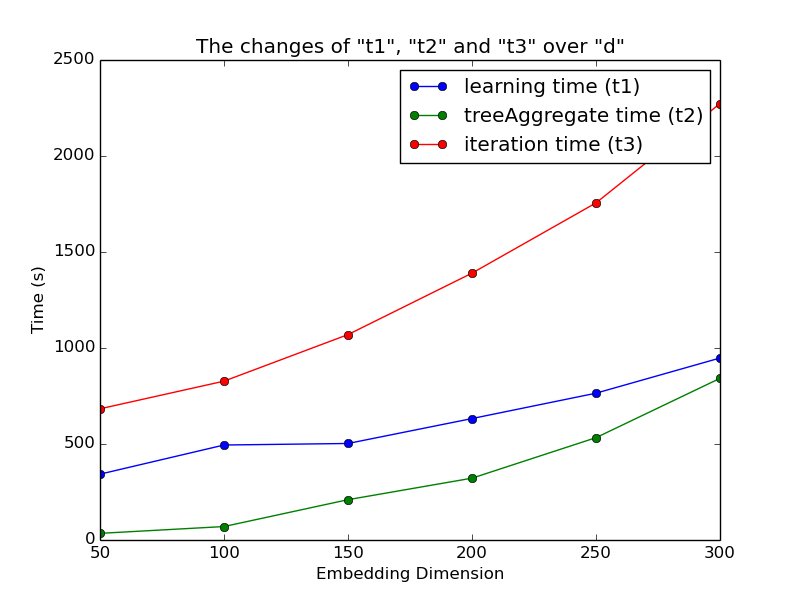
\includegraphics[width=0.8\textwidth]{vectime} 
	\caption{Shows the effect of varying embedding dimensionality of our Model on the Time}
	\label{fig:vec_time}
\end{figure}

\begin{figure}[!ht]
  \centering
	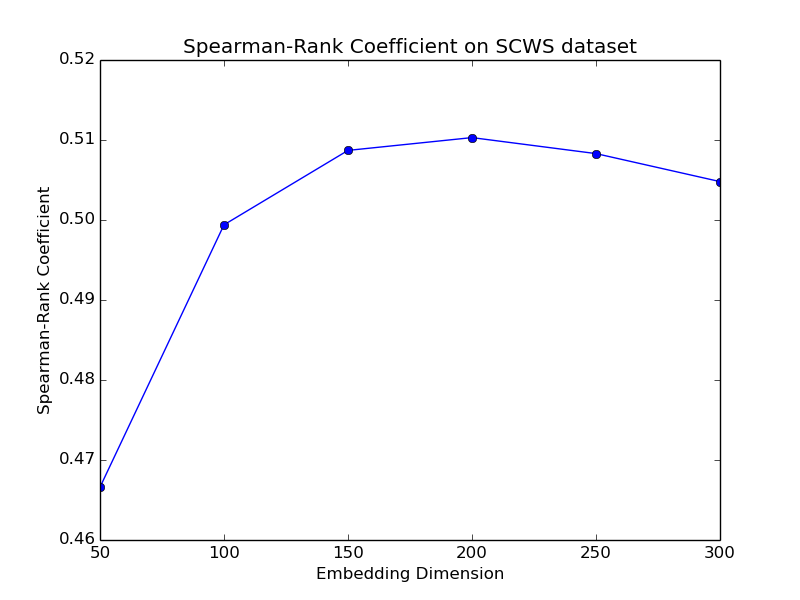
\includegraphics[width=0.7\textwidth]{vecSCWS} 
	\caption{Shows the effect of varying embedding dimensionality of our Model on the SCWS task}
	\label{fig:vec_SCWS}
\end{figure}


\begin{figure}[!ht]
  \centering
	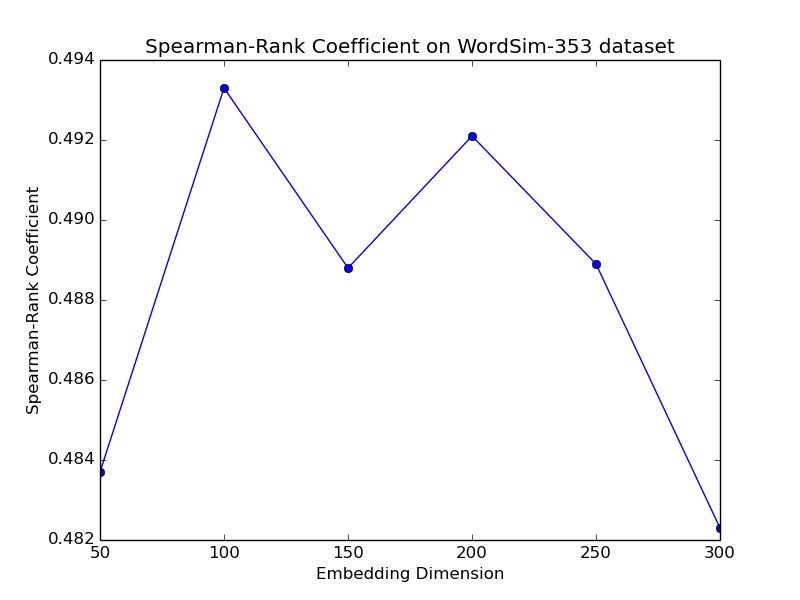
\includegraphics[width=0.7\textwidth]{vecword353} 
	\caption{Shows the effect of varying embedding dimensionality of our Model on the word353 task}
	\label{fig:vec_word353}
\end{figure}




\paragraph{Different Min Count} \ \\
We can find from Table \ref{tab:group2} , the size of dictionary is not the important factor based on loss or similarity tasks. Min count is used to remove some words which is not frequent. As we know , each word's embedding vector is trained based on the surrounding words. Since those words are infrequent, each of them involve the training of frequent words very few. So they won't affect the final embedding vectors of frequent words.

\begin{table}[H]
\caption{Different Min Count Comparison} \label{tab:group2} 
\begin{center}
\begin{tabular}{|l|l|l|l|l|l|l|l|l|l|}
\hline
id& c1 & t1 & t2 & iter & t3 & t4 & loss & SCWS & word353	   \\ 
\hline
6 	&  200 	& 342.9	& 34.6	& 35	& 683.3 &	23915  & 0.2458 &0.4666 & 0.5449  \\ 
\hline
7	&  20	& 849.0	& 343	& 35	& 1838.1 &	64335  & 0.2457 &0.4371	&0.4891    \\ 
\hline
\end{tabular}
\end{center}
\end{table}

\paragraph{Different Sense Count Comparison} \ \\
From Table \ref{tab:group3} tell us ...

\begin{table}[H]
\caption{Different Sense Count Comparison} \label{tab:group3} 
\begin{center}
\begin{tabular}{|l|l|l|l|l|l|l|l|l|l|}
\hline
id& cm & t1 & t2 & iter & t3 & t4 &    loss  & 	SCWS & 	word353	   \\ 

\hline
7	& 2000$\_$10000	& 849	& 343	& 35	& 1838 &	64335  & 0.2457 &0.4371	&0.4891	  \\ 
\hline
9 	& 2000$\_$100000 	& 798	& 338	& 35	& 1712 &	59912  & 0.2465 &0.443 & 0.498  \\ 
\hline
10 	& 7000$\_$10000 	& 808	& 340	& 35	& 1740  &	60909  & 0.2462 &0.4351 & 0.506  \\ 
\hline
\end{tabular}
\end{center}
\end{table}


\paragraph{Different Learning Rate and Gamma} \ \\
Table \ref{tab:group4} shows that ...

\begin{table}[H]

\begin{center}
\begin{tabular}{|l|l|l|l|l|l|l|l|l|l|l|}
\hline
id& lr & gm & t1 & t2 & iter & t3 & t4 &    loss  & 	SCWS & 	word353	  \\ 
\hline
7	& 0.1		& 0.9		& 849	& 343	& 35	& 1838 &	64335  & 0.246 &0.4371	&0.4891	  \\ 
\hline
8	& 0.01		& 0.95		& 797	& 370	& 40	& 1851 &	74032  & 0.267 &..	&..	  \\ 
\hline
\end{tabular}
\caption{Different Learning Rate and Gamma Comparison} \label{tab:group4} 
\end{center}
\end{table}

\paragraph{Different Syn1 Property}  \ \\
From \ref{tab:group5} , it is very obvious that if syn1 has multiple sense embeddings (output embeddings), the final loss is much smaller, although it needs more time to achieve convergence. The reason should be clear somehow. For each center word with giving sense, it has more options to choose, so the final loss is obviously trained smaller. But from the comparison of nearest words in \ref{tab:nearestcompare}, we can find that experiment 4 (multiple output embeddings) can not really split up the meaning of word senses, different senses of each word are very similar to each other based on the nearest words. This results also let us think about our model again. Maybe the output embedding should not be prototypes. But we don't have theoretical knowledge to explain such case and for now can not explain it properly. We think this can be the analysis working to do in the future. 

\begin{table}[H]

\begin{center}
\begin{tabular}{|l|l|l|l|l|l|l|l|l|l|}
\hline
id& syn1 & t1 & t2 & iter & t3 & t4 &    loss  & 	SCWS & 	word353	   \\ 
\hline
7	& true		& 849	& 343	& 35	& 1838 &	64335 & 0.2457 &0.4371	&0.4891	   \\ 
\hline
11 	& false		& 1192	& 365	& 45	& 2866 &	128949 & 0.2069 & & 0.4802  \\ 
\hline
\end{tabular}
\caption{Different Syn1 Property Comparison} \label{tab:group5} 
\end{center}
\end{table}
 

\begin{table}[H]

\begin{center}
\begin{tabular}{ |l|l|l| }
\hline
 & id 7 , one sense output embedding& id 11, multiple senses output embedding \\
\hline
\hline
\multirow{3}{*}{apple} 
 & cheap, junk, scrap, advertised 				& kodak, marketed, nokia, kit \\
 & chocolate, chicken, cherry, berry 		& portable, mgm, toy, mc \\
 & macintosh, linux, ibm, amiga			& marketed, chip, portable, packaging \\ 
 \hline
\multirow{3}{*}{bank} 
 & corporation, banking, banking, hsbc & trade, trust, venture, joint \\
 & deposit, stake, creditors, concession & trust, corporation, trade, banking \\ 
 & banks, side, edge, thames &  banks, border, banks, country \\ 
 \hline
\multirow{3}{*}{cell} 
 & imaging, plasma, neural, sensing & dna, brain, stem, virus \\
 & lab, coffin, inadvertently, tardis & cells, dna, proteins, proteins \\
 & cells, nucleus, membrane, tumor & dna, cells, plasma, fluid \\
\hline
\end{tabular}
\caption{Nearest words comparison} \label{tab:nearestcompare} 
\end{center}
\end{table}

 
\subsection{Case Analysis}

In the following, we will select only one experiment's result to do visualization and nearest words. The selection is based on the final loss and similarity task, specifically it is experiment 7 from above.  \\

Firstly we give the result from $apple$,  which is very clear. Different sense has different meanings. Table \ref{tab:sensematrixapple} shows the sense similarity matrix of $apple$. The similarity value is the cosine similarity between two embedding vectors. And table \ref{tab:nearestapple} shows the nearest words of different senses from $apple$. We can see that $apple_0$ and $apple_1$ are about food. They are similar somehow. And $apple_2$ is about company. The next are some sentence examples including $apple$ in Table \ref{tab:sentenceapple}. These are assigned sentences from the last iteration of training. To make it clear, we only display the sense label of the $apple$. We selected 100 nearest words for each sense of $apple$ and do t-SNE embedding to reduce the dimension to 2. And then we only displayed $70\%$ of words randomly to make visualization better, which is shown in Figure \ref{fig:apple}. And we use another table (Table ..) to show the comparison of with other two models (huang and em).
 
\begin{table}[H]

\begin{center} \begin{tabular}{|l|l|l|l|}  
\hline
& $apple_0$ & $apple_1$ & $apple_2$ \\ 
\hline  
$apple_0$  & 1.000000  & 0.788199 & 0.800783 \\ 
\hline 
$apple_1$  & 0.788199 & 1.000000 & 0.688523  \\ 
\hline 
$apple_2$  & 0.800783 & 0.688523 & 1.000000  \\
\hline
\end{tabular} 
\caption{Sense Matrix Of $apple$} \label{tab:sensematrixapple} 
\end{center}
\end{table}
 
 

\begin{table}[H]

\begin{center} \begin{tabular}{|l|l|}  
\hline 
$apple_0$: & cheap , junk , scrap , advertised , gum , liquor , pizza   \\  
\hline
$apple_1$: & chocolate, chicken, cherry, berry, cream, pizza, strawberry  \\  
\hline
$apple_2$: & macintosh, linux, ibm, amiga, atari, commodore, server   \\  
\hline
\end{tabular}
\caption{Nearest Words of $apple$} \label{tab:nearestapple} 
\end{center}
\end{table}


\begin{table}[H]

\begin{center} 
\begin{tabular}{|l|l|}
\hline
\multirow{2}{*}{$apple_0$} 
&he can't tell an onion from an \textcolor{red}{$apple_0$} and he's your eye witness\\
&some fruits e.g \textcolor{red}{$apple_0$} pear quince will be ground\\
\hline
\multirow{2}{*}{$apple_1$} 
&the cultivar is not to be confused with the dutch rubens \textcolor{red}{$apple_1$}\\
&the rome beauty \textcolor{red}{$apple_1$} was developed by joel gillette \\
\hline
\multirow{2}{*}{$apple_2$} 
&a list of all \textcolor{red}{$apple_2$} internal and external drives in chronological order\\
&the game was made available for the \textcolor{red}{$apple_2$} iphone os mobile platform\\
\hline
\end{tabular} 
\caption{Sentence Examples of $apple$} \label{tab:sentenceapple} 
\end{center}
\end{table}


\begin{figure}[!ht]
  \centering
	\fbox{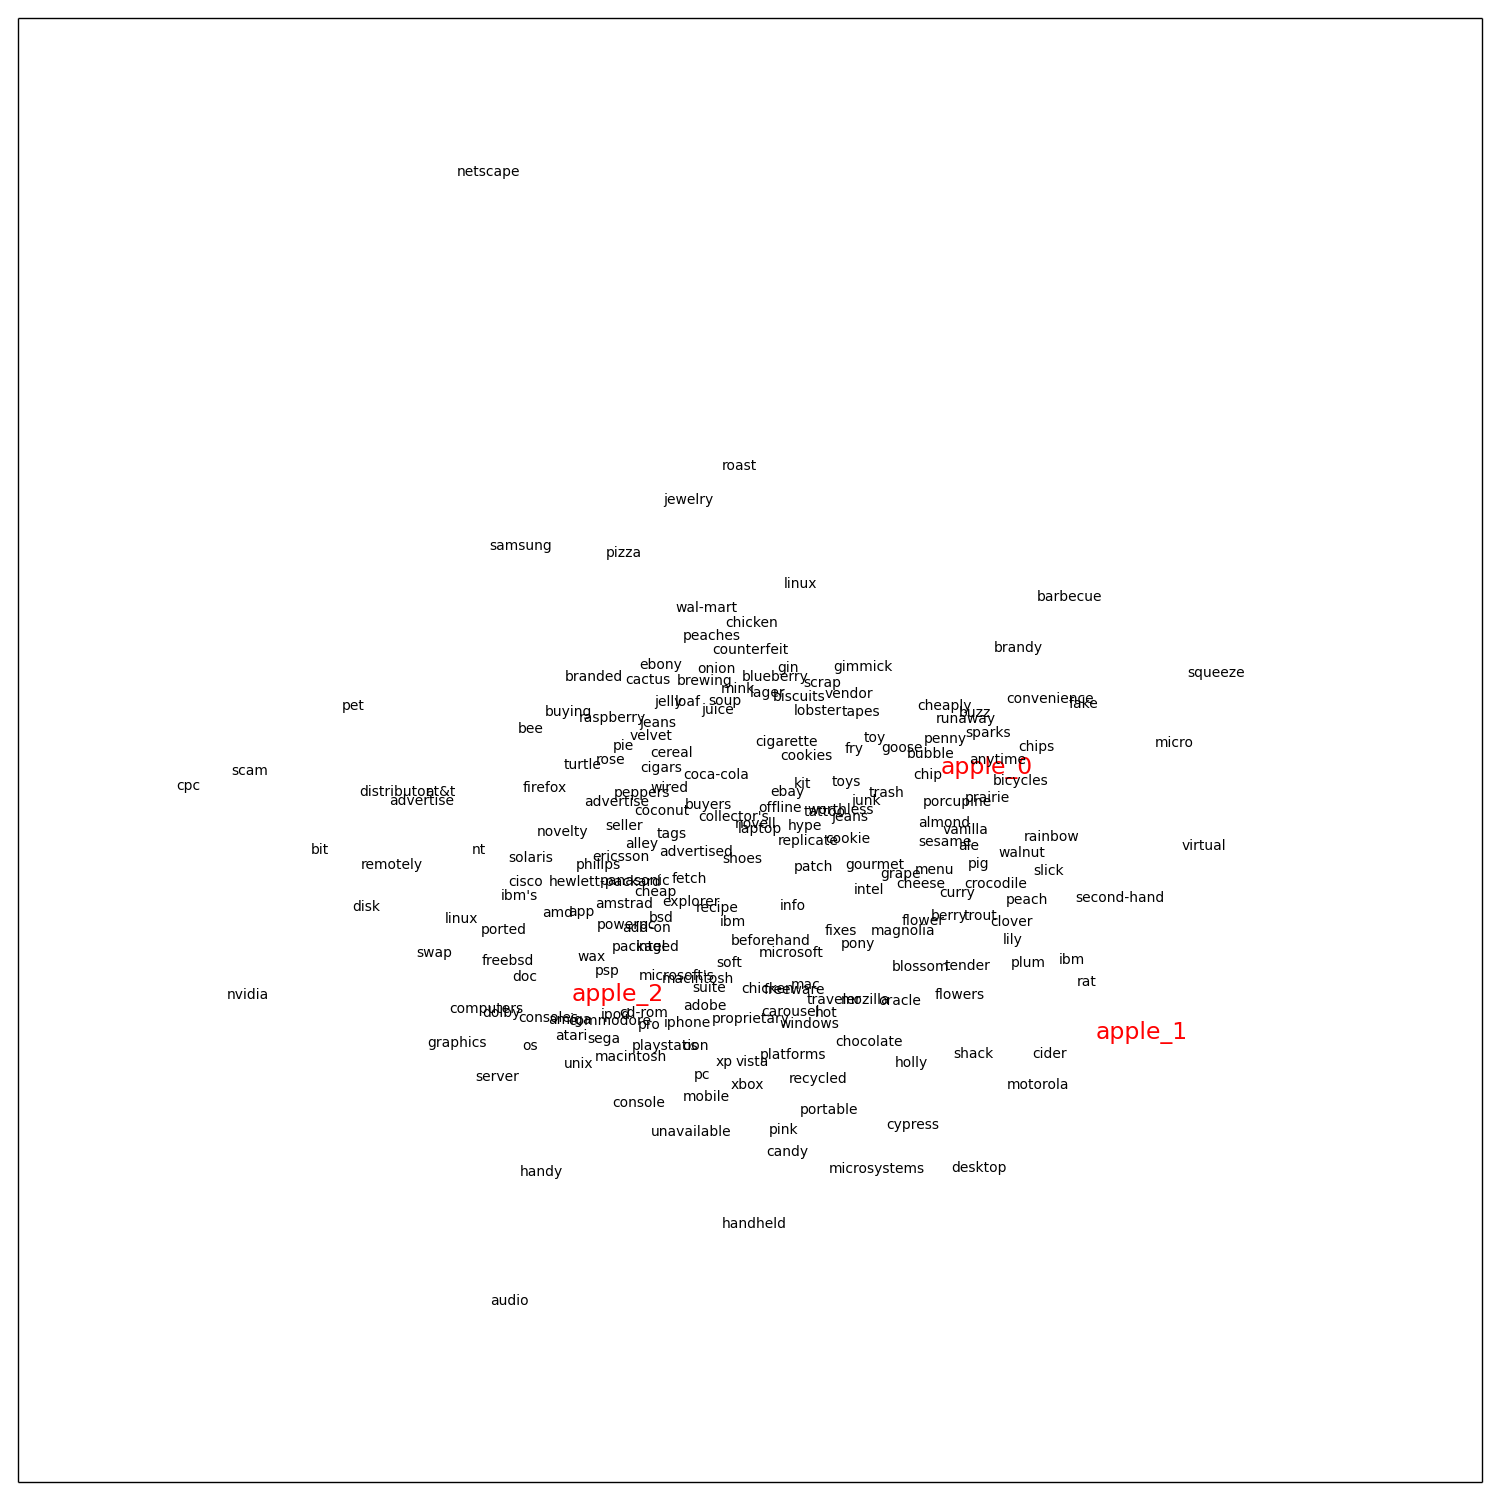
\includegraphics[width=0.8\textwidth]{apple} }
	\caption{Nearest words from $apple$}
	\label{fig:apple}
\end{figure}



\paragraph{} Next, we select other 5 words $fox$ , \ $net$ , \ $rock$ , \ and $plant$, and also list nearest words as Table .. and sentence examples as Table ... in the following. The example sentences are also cut by ourself without affecting the meaning of the sentence. It's not difficult to find that $fox$ has meanings: ; $net$ has meanings: ; $rock$ has meanings: ; $plant$ has meanings: . 


\begin{center} \begin{tabular}{l*{6}{c}r}  $fox_0$ & archie& potter& wolfe& hitchcock& conan& burnett& savage  \\ $fox_1$ & buck& housewives& colbert& eastenders& howard& kane& freeze
 \\ $fox_2$ & abc& sky& syndicated& cw& network's& ctv& pbs \\ \end{tabular} \end{center}

\begin{center} \begin{tabular}{l*{6}{c}r}   $net_0$: & generates& atm& footprint& target& kbit/s& throughput& metering   \\  $net_1$: & trillion& rs& earnings& turnover& gross& euros& profit  
 \\  $net_2$: &jumped& rolled& rebound& ladder& deficit& snapped& whistle   \\  \end{tabular} \end{center}
 
\begin{center} \begin{tabular}{l*{6}{c}r}   $rock_0$: &echo& surf& memphis& strawberry& clearwater& cliff& sunset  \\  $rock_1$: & r$\&$b& hip& roll& indie& ska& indie& hop  
 \\  $rock_2$: &formations& crust& melting& lava& boulders& granite& dust   \\  \end{tabular} \end{center}
 
 \begin{center} \begin{tabular}{l*{6}{c}r}   $run_0$: & blair& taft& fraser& monroe& precinct& mayor's& governor's  \\  $run_1$: & streak& rushing& tying& shutout& inning& wicket& kickoff
 \\  $run_2$: &running& tram& travel& express& trams& inbound& long-distance \\  \end{tabular} \end{center}
 
 \begin{center} \begin{tabular}{l*{6}{c}r}   $plant_0$: &plants& insect& seeds& seed& pollen& aquatic& organic  \\  $plant_1$: &flowering& orchid& genus& bird& species& plants& butterfly
 \\  $plant_2$: &electricity& steel& refinery& refinery& manufacturing& gas& turbine  \\  \end{tabular} \end{center}

\begin{table}
\begin{center} 
\begin{tabular}{|l|l|}
\hline
\multirow{3}{*}{$fox$} 
&run by nathaniel mellors dan \textcolor{red}{$fox_0$} andy cooke and ashley marlowe\\
&he can box like a \textcolor{red}{$fox_1$} he's as dumb as an ox\\
&the grand final was replayed on fox sports australia and the \textcolor{red}{$fox_2$} footy channel\\
\hline
\multirow{3}{*}{$net$} 
&\textcolor{red}{$net_0$} supports several disk image formats partitioning schemes\\
&in mr cook was on the forbes with a \textcolor{red}{$net_1$} worth of billion \\
&nothin but \textcolor{red}{$net_2$} freefall feet into a net below story tower\\
\hline
\multirow{3}{*}{$rock$} 
&zero nine is a finnish hard \textcolor{red}{$rock_0$} band formed in kuusamo in\\
&matt ellis b december is a folk \textcolor{red}{$rock_1$} genre singer-songwriter\\
&cabo de natural park is characterised by volcanic \textcolor{red}{$rock_2$} formations\\
\hline
\multirow{3}{*}{$run$} 
&dean announced that she intends to \textcolor{red}{$run_0$} for mayor again in the november election\\
& we just couldn't \textcolor{red}{$run_1$} the ball coach tyrone willingham said\\
& the terminal is \textcolor{red}{$run_2$} by british rail freight company ews\\
\hline
\multirow{3}{*}{$plant$} 
&these phosphoinositides are also found in \textcolor{red}{$plant_0$} cells with the exception of pip\\
&is a genus of flowering \textcolor{red}{$plant_1$} in the malvaceae sensu lato\\
&was replaced with a new square-foot light fixture \textcolor{red}{$plant_2$} in sparta tn\\
\hline
\end{tabular} 
\caption{Sentence Examples of $apple$} \label{tab:sentenceapple} 
\end{center}
\end{table}


\paragraph{} In the last, for each sense of each word ($apple$, $fox$,$net$,$rock$ and $plant$), we select only 20 nearest words, and combine them together to do another t-SNE embedding, which is also two dimension. The the result is shown in Figure \ref{fig:keywords20}. 

\begin{figure}[!ht]
  \centering
	\fbox{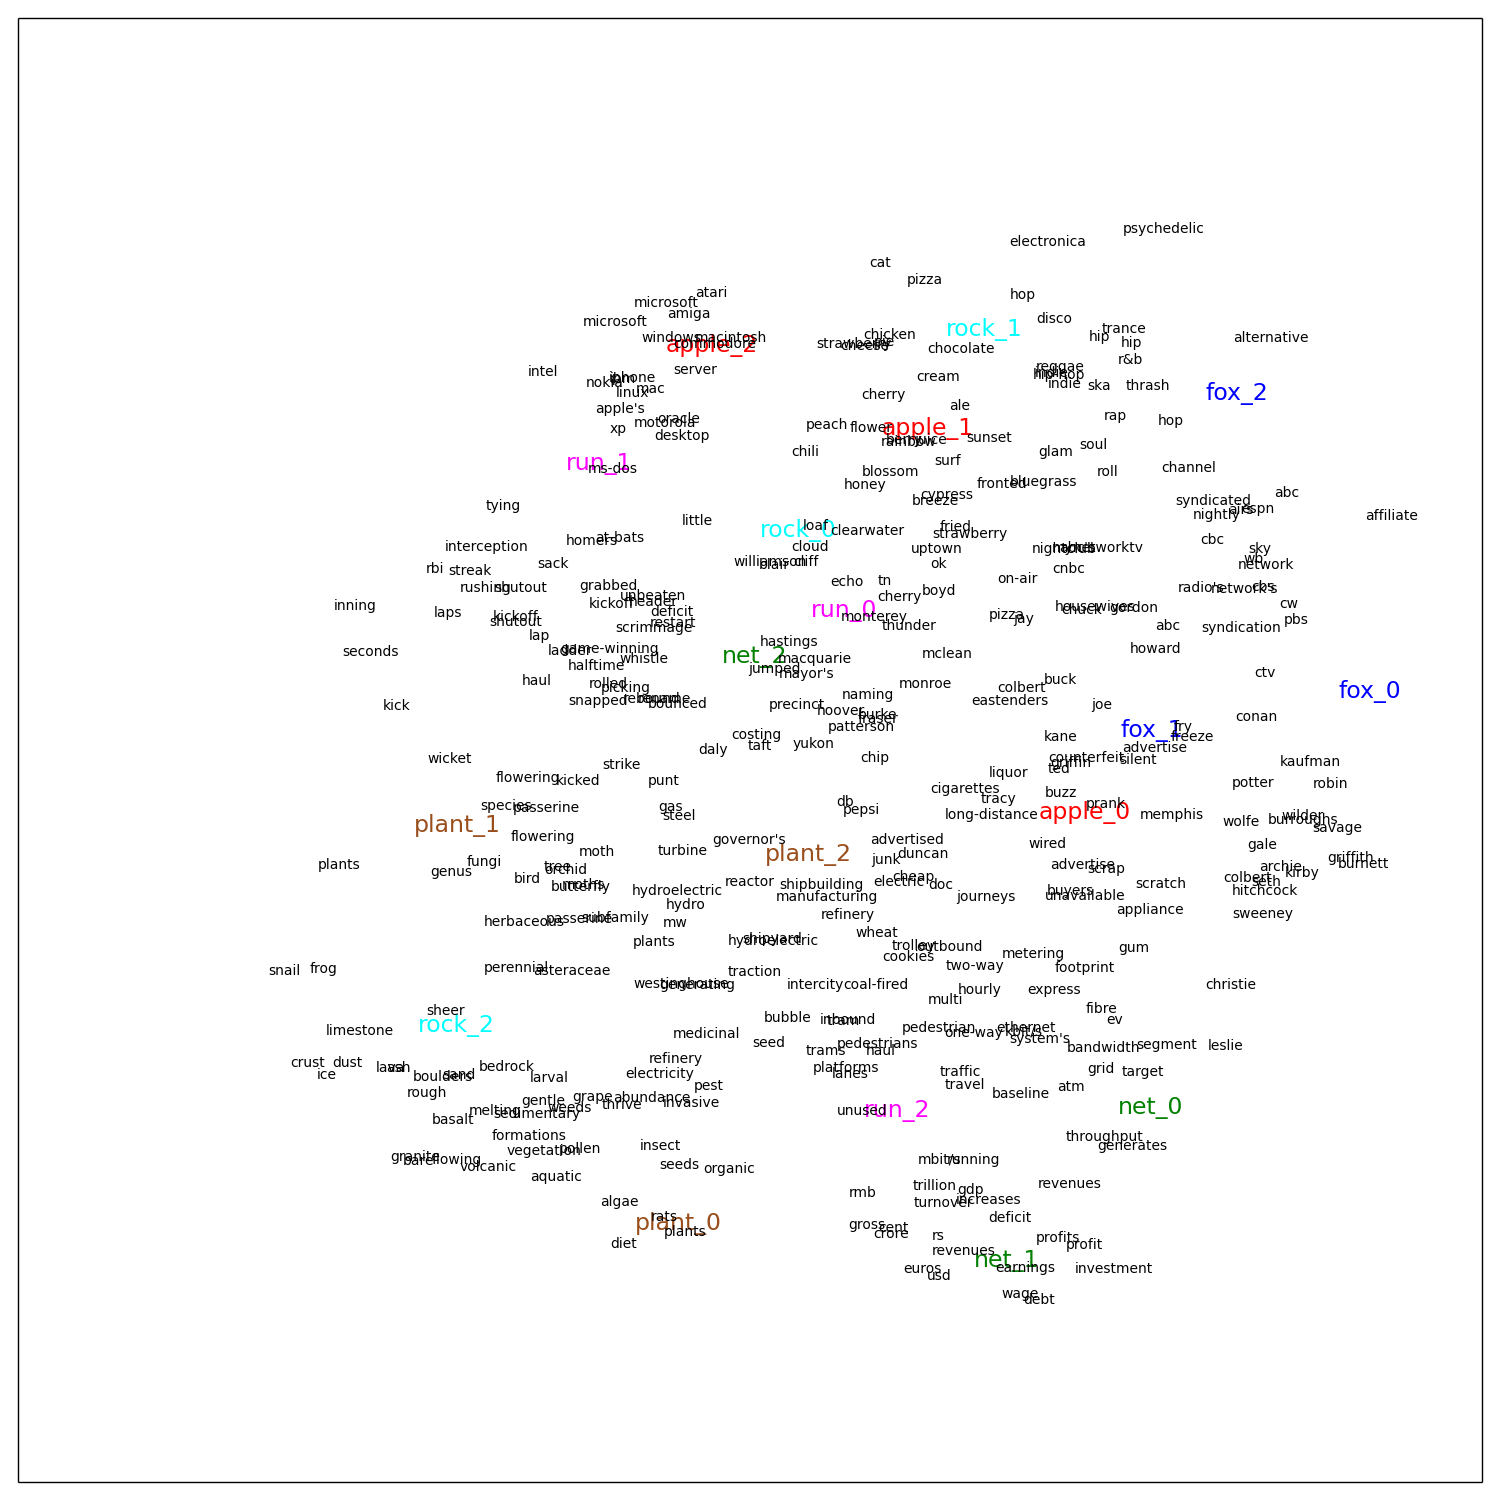
\includegraphics[width=0.9\textwidth]{some20} }
	\caption{Nearest words from 5 key words: $apple$,\ ,$fox$,\ ,$net$,\ ,$rock$,\  , $run$ and $plant$}
	\label{fig:keywords20}
\end{figure}

\paragraph{} From the above results, we can say our model is successful to get multiple senses vectors.


\chapter{Conclusion}
\label{cha:concl}

My master thesis provides an approach for the inventor identification by using clustering algorithms combined with the logistic regression and the patent-publication matching. The approach first extends the Fleming's inventor-patent instance data structure by adding four text features. Different methods are designed to calculate the similarities based on different features. With a training dataset, the approach uses the logistic regression to assign each feature similarity a suitable weight and find a suitable threshold to decide if two inventor-patent instances are from the same inventor. The DBSCAN and the hierarchical clustering try to group the inventor-patent instances from the same inventor and perform the transitivity for the inventor identity. The clustering algorithms make use of the weights and the threshold generated by the logistic regression. Some optimization techniques such as LSI, the "Bold-driver" technique and the "Stop-early" technique are used for optimizations. From the evaluation result, the clustering algorithms combined with the logistic regression show good performances for the inventor identification. Because of the good performances of clustering algorithms and the incomplete information provided by the publication database, the patent-publication matching doesn't help to improve the accuracy. In conclusion, the approach has a good ability to do the inventor identification.
\newline

There are several directions for the future work. If the approach is going to be applied on another patent database, a representative training dataset should be prepared for the logistic regression. The training dataset is generated from the inventor-patent instance dataset which contains $\frac{n(n-1)}{2}$ pieces of data where $n$ is the number of inventor-patent instances. Some techniques such as the mini-batch gradient descent method or the stochastic gradient descent method can be used to accelerate the training process when the size of the training dataset becomes large. From the evaluation, the single linkage clustering and the minPts with 1 show the best performances. Both of them make the transitivity into a high level. The transitivity as a high level aims at decreasing the \emph{splitting} error. But in the future, more and more inventors would have the same name. Keeping the transitivity as a high level may result in a bigger \emph{lumping} error. Except finding a better training dataset, the method to calculate the similarities between clusters and the value of minPts should also be adjusted again to find the best performance. 

\newpage
\thispagestyle{empty}
\rule{0cm}{5cm}

%Although the patent-publication matching doesn't help to improve the accuracy during the evaluation process, it is still promising to be helpful if a good publication database can be found.




\chapter{Appendix}
\label{cha:appendix}

% References
%
% There many ways to get a bibliography style
% 1. Use thesis.bst as included in this package (reasonable layout)
% 2. Customize thesis.dbj and rerun "latex thesis.dbj" to produce a new thesis.bst
%    (for experienced user)
% 3. Run "tex makebst.tex" (using makebst.tex from the custom-bib package) to create your own DBJ & BST-file
%    (for the very experienced user)
% 4. Code your BST file from scratch (for the BibTeX nerd)

% thesis.bst as included should be a good start, though
\bibliographystyle{thesis}

% Use bibtex to manage your references
% Jabref is a useful tool for editing a bibtex file
% The bibtex file modelman.bib included in this template
% is a snapshot of the main bibtex file of the group.
% The most recent version is in the CVS directory papers/bib
% In any case, give complete information about the references:
% Authors, title, place of publication (conference,journal),
% Year of publication, page numbers, URL if the document is
% also available online.
\bibliography{modelman}









\bibliographystyle{apalike}
\bibliography{deepLearn16}



\end{document}


